% Author: Izaak Neutelings (October 2021)
% Inspiration
%   "Very special relativity - An illustrated guide", Sander Bais (2007)
%   http://people.uncw.edu/hermanr/GR/Minkowski/Minkowski.pdf
\documentclass[border=3pt,tikz]{standalone}
\usepackage{amsmath} % for \text
\usepackage{etoolbox} % ifthen
\usepackage[outline]{contour} % glow around text
\usetikzlibrary{calc} % for adding up coordinates
\usetikzlibrary{decorations.markings,decorations.pathmorphing}
\usetikzlibrary{angles,quotes} % for pic (angle labels)
\usetikzlibrary{arrows.meta} % for arrow size
\usepackage{xfp} % higher precision (16 digits?)
\contourlength{1.1pt}

\tikzset{>=latex} % for LaTeX arrow head
\colorlet{myred}{red!85!black}
\colorlet{mydarkred}{red!55!black}
\colorlet{mylightred}{red!85!black!12}
\colorlet{myfieldred}{mydarkred!5} % for S' background
\colorlet{myredhighlight}{myred!20} % highlights simultaneity in ladder paradox
\colorlet{myblue}{blue!80!black}
\colorlet{mydarkblue}{blue!50!black}
\colorlet{mylightblue}{blue!50!black!30}
\colorlet{mylightblue2}{myblue!10}
\colorlet{mygreen}{green!80!black}
\colorlet{mypurple}{blue!40!red!80!black}
\colorlet{mydarkgreen}{green!50!black}
\colorlet{mydarkpurple}{blue!40!red!50!black}
\colorlet{myorange}{orange!40!yellow!95!black}
\colorlet{mydarkorange}{orange!40!yellow!85!black}
\colorlet{mybrown}{brown!20!orange!90!black}
\colorlet{mydarkbrown}{brown!20!orange!55!black}
\colorlet{mypurplehighlight}{mydarkpurple!20} % highlights simultaneity in ladder paradox
\tikzstyle{world line}=[myblue!40,line width=0.3]
\tikzstyle{world line t}=[mypurple!50!myblue!40,line width=0.3]
\tikzstyle{world line'}=[mydarkred!40,line width=0.3]
\tikzstyle{mysmallarr}=[-{Latex[length=3,width=2]},thin]
\tikzstyle{mydashed}=[dash pattern=on 3 off 3]
\tikzstyle{rod}=[mydarkbrown,draw=mydarkbrown,double=mybrown,double distance=2pt,
                 line width=0.2,line cap=round,shorten >=1pt,shorten <=1pt]
%\tikzstyle{rod'}=[rod,draw=mydarkbrown!80!red!85,double=mybrown!80!red!85]
\tikzstyle{vector}=[->,line width=1,line cap=round]
\tikzstyle{vector'}=[vector,shorten >=1.2]
\tikzstyle{particle}=[mygreen,line width=0.9]
\tikzstyle{photon}=[-{Latex[length=5,width=4]},myorange,line width=0.8,decorate,
                    decoration={snake,amplitude=1.0,segment length=5,post length=5}]

\def\tick#1#2{\draw[thick] (#1) ++ (#2:0.06) --++ (#2-180:0.12)}
\def\tickp#1#2{\draw[thick,mydarkred] (#1) ++ (#2:0.06) --++ (#2-180:0.12)}
\def\Nsamples{100} % number samples in plot

\begin{document}


% SPACETIME DIAGRAM
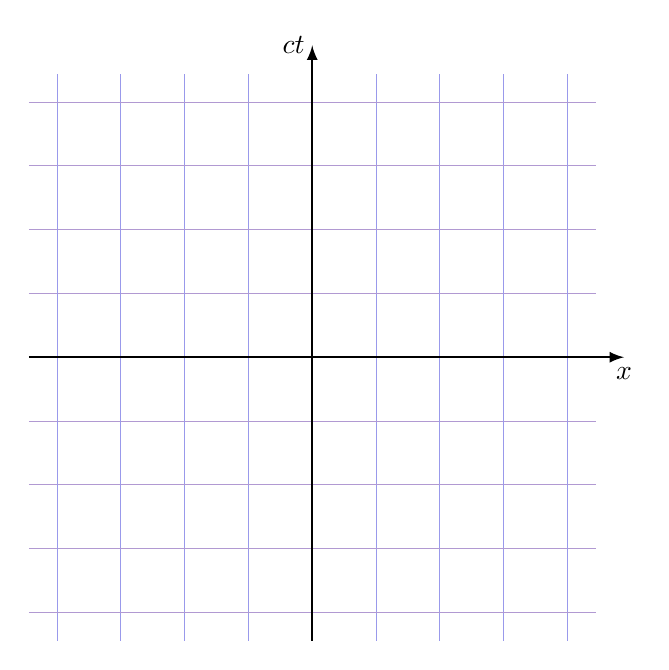
\begin{tikzpicture}[scale=1.8]
  \message{Basic spacetime diagram^^J}
  
  \def\xmax{2}
  \def\Nlines{4} % number of world lines (at constant x/t)
  
  % WORLD LINES GRID
  \message{  Making world lines...^^J}
  \foreach \i [evaluate={\x=\i*0.9*\xmax/\Nlines;}] in {1,...,\Nlines}{
    \message{  Running i/N=\i/\Nlines, x=\x...^^J}
    \draw[world line]   (-\x,-\xmax) -- (-\x,\xmax);
    \draw[world line]   ( \x,-\xmax) -- ( \x,\xmax);
    \draw[world line t] (-\xmax,-\x) -- (\xmax,-\x);
    \draw[world line t] (-\xmax, \x) -- (\xmax, \x);
  }
  
  % AXES
  \draw[->,thick] (0,-\xmax) -- (0,\xmax+0.2) node[left=-1] {$ct$};
  \draw[->,thick] (-\xmax,0) -- (\xmax+0.2,0) node[below=0] {$x$};
  
\end{tikzpicture}


% SPACETIME DIAGRAM with WORLD LINES
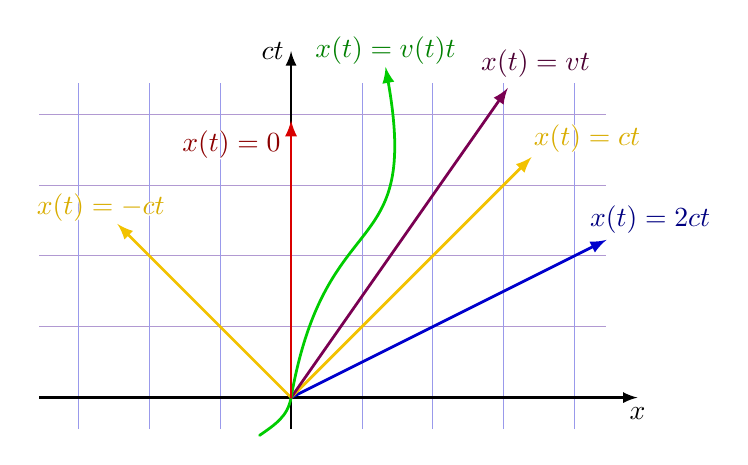
\begin{tikzpicture}[scale=2.0]
  \message{Worldlines^^J}
  
  \def\ymin{0.2}
  \def\xmin{1.6}
  \def\xmax{2}
  \def\Nlines{4} % number of world lines (at constant x/t)
  \pgfmathsetmacro\d{0.9*\xmax/\Nlines} % grid size
  \coordinate (O) at (0,0);
  \coordinate (T) at (0,\xmax+0.2);
  
  % WORLD LINES GRID
  \message{  Making world lines...^^J}
  \foreach \i [evaluate={\x=\i*\d;}] in {1,...,\Nlines}{
    \message{  Running i/N=\i/\Nlines, x=\x...^^J}
    \draw[world line]   ( \x,-\ymin) -- ( \x,\xmax);
    \draw[world line t] (-\xmin, \x) -- (\xmax, \x);
  }
  \draw[world line] (-\d,-\ymin) -- (-\d,\xmax);
  \draw[world line] (-2*\d,-\ymin) -- (-2*\d,\xmax);
  \draw[world line] (-3*\d,-\ymin) -- (-3*\d,\xmax);
  
  % AXES
  \draw[->,thick] (0,-\ymin) -- (T) node[left=-1] {$ct$};
  \draw[->,thick] (-\xmin,0) -- (\xmax+0.2,0) node[below=0] {$x$};
  
  % VECTORS
  \draw[vector,myorange] (O) -- (135:0.78*\xmax)
    node[mydarkorange,left=6,above=-3] {\contour{white}{$x(t)=-ct$}};
  \draw[vector,myblue] (O) -- ({atan(1/2)}:1.12*\xmax) %(45/2:\xmax)
    node[mydarkblue,anchor=-155,outer sep=-1] {$x(t)=2ct$};
  \draw[vector,myorange] (O) -- (45:1.08*\xmax)
    node[mydarkorange,left=1,above right=-2] {\contour{white}{$x(t)=ct$}};
  \draw[vector,mypurple] (O) -- (55:1.2*\xmax)
    node[mydarkpurple,right=10,above] {\contour{white}{$x(t)=vt$}};
  \draw[vector,mygreen]
    (-0.10*\xmax,-0.12*\xmax) to[out=35,in=-100] (O)
    to[out=80,in=-80,looseness=1.5] (0.3*\xmax,1.05*\xmax)
    node[mydarkgreen,above=-3] {\contour{white}{$x(t)=v(t)t$}};
  \draw[vector,myred] (O) -- (0,0.88*\xmax)
    node[mydarkred,below left=0] {\contour{white}{$x(t)=0$}};
  %\node[right=8,above,mydarkpurple] at (T) {$x(t)=0$};
  
\end{tikzpicture}


% SPACETIME DIAGRAM with TWO OBSERVERS
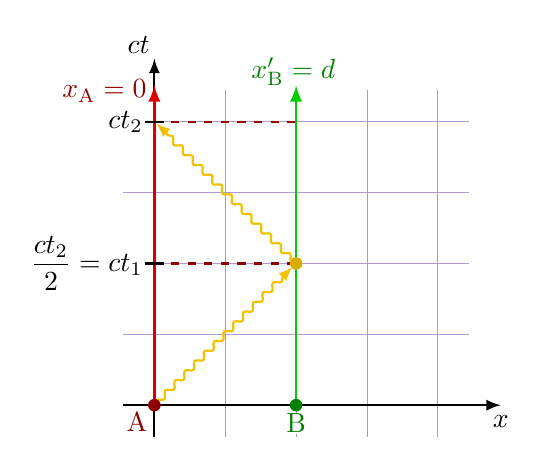
\begin{tikzpicture}[scale=2.0]
  \message{Two observers^^J}
  
  \def\xmin{0.2}
  \def\xmax{2}
  \def\R{2.03} % vector length
  \def\Nlines{4} % number of world lines (at constant x/t)
  \pgfmathsetmacro\d{0.9*\xmax/\Nlines} % grid size
  \pgfmathsetmacro\D{2*\d} % distance between observers
  \coordinate (A) at (0,0); % observer A at t=0
  \coordinate (B) at (\D,0); % observer B at t=0
  \coordinate (C) at (2*\d,2*\d); % point of reflection
  \coordinate (T1) at (0,2*\d); % time of reflection
  \coordinate (T2) at (0,4*\d); % light returning at x=0
  
  % WORLD LINES GRID
  \message{  Making world lines...^^J}
  \foreach \i [evaluate={\x=\i*\d;}] in {1,...,\Nlines}{
    \message{  Running i/N=\i/\Nlines, x=\x...^^J}
    \draw[world line]   ( \x,-\xmin) -- ( \x,\xmax);
    \draw[world line t] (-\xmin, \x) -- (\xmax, \x);
  }
  
  % AXES
  \draw[->,thick] (0,-\xmin) -- (0,\xmax+0.2) node[above left=-2] {$ct$};
  \draw[->,thick] (-\xmin,0) -- (\xmax+0.2,0) node[below=0] {$x$};
  \draw[thick,mydarkred,dashed] (T1) -- (C);
  \draw[thick,mydarkred,dashed] (T2) -- (2*\d,4*\d);
  
  % VECTORS
  \draw[vector,myred] (A) --++ (0,\R)
    node[mydarkred,above=-2,left=-1] {\contour{white}{$x_\mathrm{A}=0$}};
  \draw[vector,mygreen] (B) --++ (0,\R)
    node[mydarkgreen,left=1,above=-4] {\contour{white}{$x_\mathrm{B}'=d$}};
  \draw[photon,shorten >=1] (C) -- (T2);
  \fill[mydarkorange] (C) circle(0.04);
  \draw[photon,shorten >=2] (A) -- (C);
  \fill[mydarkred] (A) circle(0.04) node[below left=-1] {A}; % observer A
  \fill[mydarkgreen] (B) circle(0.04) node[fill=white,inner sep=0.5,below=2.5] {B}; % observer B
  
  % TICKS
  \node[fill=white,inner sep=1,left=3] at (T1) {$\dfrac{ct_2}{2}=ct_1$};
  \node[fill=white,inner sep=1,left=3] at (T2) {$ct_2$};
  \tick{T1}{0};
  \tick{T2}{0};
  
\end{tikzpicture}


% SPACETIME DIAGRAM with TWO MOVING OBSERVERS to show simultaneity
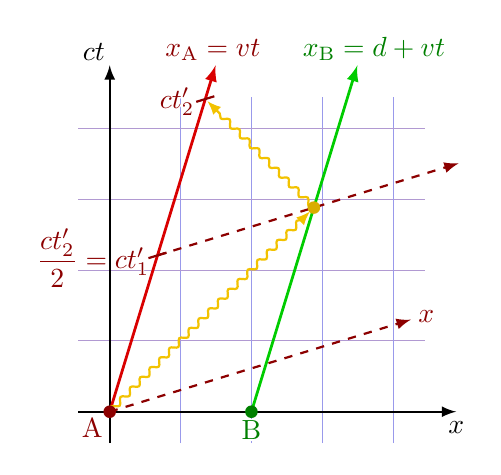
\begin{tikzpicture}[scale=2.0]
  \message{Two moving observers^^J}
  
  \def\xmin{0.2}
  \def\xmax{2}
  \def\R{2.3} % vector length
  \def\Nlines{4} % number of world lines (at constant x/t)
  \pgfmathsetmacro\ang{73} % angle between ct and ct' axes
  \pgfmathsetmacro\d{0.9*\xmax/\Nlines} % grid size
  \pgfmathsetmacro\D{2*\d} % distance between observers
  \coordinate (A) at (0,0); % observer A at t=0
  \coordinate (B) at (\D,0); % observer B at t=0
  \coordinate (C) at (45:{\D*sqrt(2)/(1-cot(\ang))}); % point of reflection
  %\coordinate (T1) at (\ang:{2*\d/sin(\ang)/sqrt(1-cot(\ang)^2)}); % time of reflection
  \coordinate (T1) at (\ang:{\D*sqrt(cot(\ang)^2+1)/(1-cot(\ang)^2)}); % time of reflection
  \coordinate (T2) at (\ang:{2*\D*sqrt(cot(\ang)^2+1)/(1-cot(\ang)^2)}); % time of reflection
  
  % WORLD LINES GRID
  \message{  Making world lines...^^J}
  \foreach \i [evaluate={\x=\i*\d;}] in {1,...,\Nlines}{
    \message{  Running i/N=\i/\Nlines, x=\x...^^J}
    \draw[world line]   ( \x,-\xmin) -- ( \x,\xmax);
    \draw[world line t] (-\xmin, \x) -- (\xmax, \x);
  }
  
  % AXES
  \draw[->,thick] (0,-\xmin) -- (0,\xmax+0.2) node[above left=-2] {$ct$};
  \draw[->,thick] (-\xmin,0) -- (\xmax+0.2,0) node[below=0] {$x$};
  \draw[->,thick,mydarkred,dashed] (A) -- (90-\ang:\xmax) node[above=1,right=-1] {$x$}; %_\mathrm{A}'
  \draw[->,thick,mydarkred,dashed] (T1) --++ (90-\ang:\xmax);
  
  % VECTORS
  \draw[vector,myred] (A) --++ (\ang:\R)
    node[mydarkred,left=1,above=-2] {$x_\mathrm{A}=vt$};
  \draw[vector,mygreen] (B) --++ (\ang:\R)
    node[mydarkgreen,right=6,above=-2] {$x_\mathrm{B}=d+vt$};
  \draw[photon,shorten >=1] (C) --++ (135:{\D*sqrt(2)/(1+cot(\ang))});
  \fill[mydarkorange] (C) circle(0.04);
  \draw[photon,shorten >=2] (A) -- (C);
  \fill[mydarkred] (A) circle(0.04) node[below left=-1] {A}; % observer A
  \fill[mydarkgreen] (B) circle(0.04) node[fill=white,inner sep=0.5,below=2.5] {B}; % observer B
  
  % TICKS
  %\node[fill=white,inner sep=1,left=3] at (T1) {$\dfrac{ct_2}{2}=ct_1$};
  %\node[fill=white,inner sep=1,left=3] at (T2) {$ct_2$};
  \tickp{T1}{90-\ang} node[left=-4] {\contour{white}{$\dfrac{ct_2'}{2}=ct_1'$}};
  \tickp{T2}{90-\ang} node[left=-3] {\contour{white}{$ct_2'$}};
  
\end{tikzpicture}


% SPACETIME DIAGRAM - LIGHT CONE
\begin{tikzpicture}[scale=1.8]
  \message{Light cone^^J}
  
  \def\xmax{2}
  \def\xmaxp{2.2} % maximum of rotated axis
  \def\Nlines{5} % number of world lines (at constant x/t)
  \pgfmathsetmacro\d{0.9*\xmax/\Nlines} % grid size
  \pgfmathsetmacro\ang{atan(1/3)} % angle between x and x' axes
  \coordinate (O) at (0,0);
  \coordinate (X) at (\xmax+0.2,0);
  \coordinate (T) at (0,\xmax+0.2);
  
  % WORLD LINE GRID
  \message{  Making world lines...^^J}
  \foreach \i [evaluate={\x=\i*\d;}] in {1,...,\Nlines}{
    \message{  Running i/N=\i/\Nlines, x=\x...^^J}
    \draw[world line]   (-\x,-\xmax) -- (-\x,\xmax);
    \draw[world line]   ( \x,-\xmax) -- ( \x,\xmax);
    \draw[world line t] (-\xmax,-\x) -- (\xmax,-\x);
    \draw[world line t] (-\xmax, \x) -- (\xmax, \x);
  }
  
  % AXES
  \draw[->,thick] (0,-\xmax) -- (T) node[left=-1] {$ct$};
  \draw[->,thick] (-\xmax,0) -- (X) node[below=0] {$x$};
  
  % LABELS
  \draw pic[->,"$45^\circ$",draw=black,angle radius=23,angle eccentricity=1.38] {angle = X--O--C};
  \node[mydarkorange,above right] at (0.1*\xmax,\xmax) {future light cone};
  \node[mydarkorange,below] at (0,-\xmax) {past light cone};
  
  % FILLS
  \fill[myblue,opacity=0.05] % SPACELIKE
    (\xmax,\xmax) -- (-\xmax,-\xmax) -- (-\xmax,\xmax) -- (\xmax,-\xmax) -- cycle;
  \fill[myorange,opacity=0.05] % TIMELIKE
    (\xmax,\xmax) -- (-\xmax,\xmax) -- (\xmax,-\xmax) -- (-\xmax,-\xmax) -- cycle;
  \node[mydarkblue,right,align=center] at (-\xmax,0.18*\xmax)
    {\contour{myblue!5}{spacelike}\\[-2]\contour{myblue!5}{region}};
  \node[mydarkblue,left,align=center] at (\xmax,0.18*\xmax)
    {\contour{myblue!5}{spacelike}\\[-2]\contour{myblue!5}{region}};
  \node[mydarkorange,align=center] at (-0.22*\xmax,0.67*\xmax)
    {\contour{myorange!5}{timelike}\\[-2]\contour{myorange!5}{region}};
  \node[mydarkorange,align=center] at (0.22*\xmax,-0.67*\xmax)
    {\contour{myorange!5}{timelike}\\[-2]\contour{myorange!5}{region}};
  
  % PHOTON
  \draw[photon] ( \xmax,-\xmax) -- ( 0.02*\xmax,-0.02*\xmax);
  \draw[photon] (-\xmax,-\xmax) -- (-0.02*\xmax,-0.02*\xmax);
  \draw[photon] ( 0.02*\xmax,0.02*\xmax) -- ( \xmax,\xmax)
    node[mydarkorange,above right] {$x=ct$};
  \draw[photon] (-0.02*\xmax,0.02*\xmax) -- (-\xmax,\xmax);
  
  % PARTICLE WORLDLINE
  \draw[particle,decoration={markings,mark=at position 0.27 with {\arrow{latex}},
                                      mark=at position 0.76 with {\arrow{latex}}},postaction={decorate}]
      (-0.5*\xmax,-\xmax) to[out=80,in=-110] (O) to[out=70,in=-100] (0.45*\xmax,\xmax);
  \fill[mydarkgreen] (O) circle(0.04); % event
  
\end{tikzpicture}


% SPACETIME DIAGRAM - VECTORS
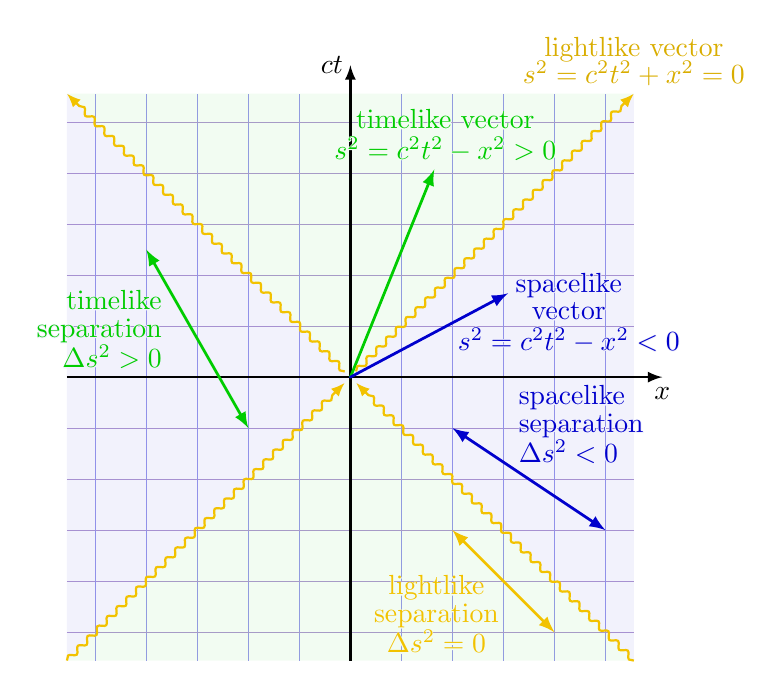
\begin{tikzpicture}[scale=1.8]
  \message{Vectors^^J}
  
  \def\xmax{2}
  \def\xmaxp{2.2} % maximum of rotated axis
  \def\Nlines{5} % number of world lines (at constant x/t)
  \pgfmathsetmacro\d{0.9*\xmax/\Nlines} % grid size
  \pgfmathsetmacro\ang{atan(1/3)} % angle between x and x' axes
  \coordinate (O) at (0,0);
  \coordinate (X) at (\xmax+0.2,0);
  \coordinate (T) at (0,\xmax+0.2);
  
  % WORLD LINE GRID
  \message{  Making world lines...^^J}
  \foreach \i [evaluate={\x=\i*\d;}] in {1,...,\Nlines}{
    \message{  Running i/N=\i/\Nlines, x=\x...^^J}
    \draw[world line]   (-\x,-\xmax) -- (-\x,\xmax);
    \draw[world line]   ( \x,-\xmax) -- ( \x,\xmax);
    \draw[world line t] (-\xmax,-\x) -- (\xmax,-\x);
    \draw[world line t] (-\xmax, \x) -- (\xmax, \x);
  }
  
  % FILLS
  \fill[myblue,opacity=0.05] % SPACELIKE
    (\xmax,\xmax) -- (-\xmax,-\xmax) -- (-\xmax,\xmax) -- (\xmax,-\xmax) -- cycle;
  \fill[mygreen,opacity=0.05] % TIMELIKE
    (\xmax,\xmax) -- (-\xmax,\xmax) -- (\xmax,-\xmax) -- (-\xmax,-\xmax) -- cycle;
  
  % AXES
  \draw[->,thick] (0,-\xmax) -- (T) node[left=-1] {$ct$};
  \draw[->,thick] (-\xmax,0) -- (X) node[below=0] {$x$};
  
  % VECTORS
  \draw[vector,mygreen] (O) --++ (68:0.79*\xmax)
    node[right=4,above=-1,align=center]
    {\contour{mygreen!5}{timelike vector}\\[-1]
     \contour{mygreen!5}{$s^2=c^2t^2-x^2>0$}};
  \draw[vector,myblue] (O) --++ (28:0.63*\xmax)
    node[below=7,right=-22,align=center]
    {\contour{myblue!5}{spacelike}\\[-2]
     \contour{myblue!5}{vector}\\[-1]
     \contour{myblue!5}{$s^2=c^2t^2-x^2<0$}};
  \draw[vector,mygreen,<->] (-2*\d,-\d) --++ (-2*\d,3.5*\d)
    node[pos=0.8,below left=-2,align=right]
    {\contour{myblue!5}{timelike}\\[-2]
     \contour{myblue!5}{separation}\\[-1]
     \contour{myblue!5}{$\Delta s^2>0$}};
  \draw[vector,myblue,<->] (2*\d,-\d) --++ (3*\d,-2*\d)
    node[pos=0.4,above right=-2,align=left]
    {\contour{myblue!5}{spacelike}\\[-2]
     \contour{myblue!5}{separation}\\[-1]
     \contour{myblue!5}{$\Delta s^2<0$}};
  \draw[vector,myorange,<->] (2*\d,-3*\d) --++ (2*\d,-2*\d)
    node[pos=0.45,below left=-4,align=center]
    {\contour{mygreen!5}{lightlike}\\[-2]
     \contour{mygreen!5}{separation}\\[-1]
     \contour{mygreen!5}{$\Delta s^2 = 0$}};
  
  % PHOTON
  \draw[photon] ( \xmax,-\xmax) -- ( 0.02*\xmax,-0.02*\xmax);
  \draw[photon] (-\xmax,-\xmax) -- (-0.02*\xmax,-0.02*\xmax);
  \draw[photon] ( 0.02*\xmax,0.02*\xmax) -- ( \xmax,\xmax)
    node[mydarkorange,above=-1,align=center] {lightlike vector\\[-2]$s^2=c^2t^2+x^2=0$};
  \draw[photon] (-0.02*\xmax,0.02*\xmax) -- (-\xmax,\xmax);
  
\end{tikzpicture}


% SPACETIME DIAGRAM - OVERLAPPING LIGHT CONES
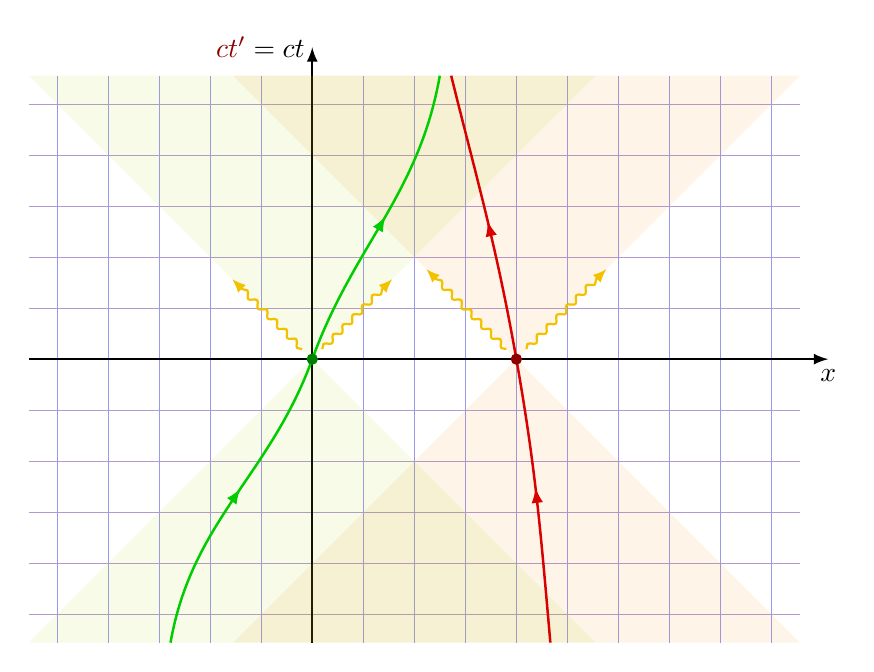
\begin{tikzpicture}[scale=1.8]
  \message{Overlapping light cones^^J}
  
  \def\xmax{2}
  \def\ext{4*\d} % extension x axis
  \def\xmaxp{2.2} % maximum of rotated axis
  \def\Nlines{5} % number of world lines (at constant x/t)
  \pgfmathsetmacro\d{0.9*\xmax/\Nlines} % grid size
  \pgfmathsetmacro\ang{atan(1/3)} % angle between x and x' axes
  \coordinate (O) at (0,0);
  \coordinate (X) at (\xmax+\ext+0.2,0);
  \coordinate (T) at (0,\xmax+0.2);
  \coordinate (B) at (4*\d,0); % event B
  
  % WORLD LINE GRID
  \message{  Making world lines...^^J}
  \foreach \i [evaluate={\x=\i*\d;}] in {1,...,\Nlines}{
    \message{  Running i/N=\i/\Nlines, x=\x...^^J}
    \draw[world line]   (-\x,-\xmax) -- (-\x,\xmax);
    \draw[world line]   ( \x,-\xmax) -- ( \x,\xmax);
    \draw[world line t] (-\xmax,-\x) -- (\xmax+\ext,-\x);
    \draw[world line t] (-\xmax, \x) -- (\xmax+\ext, \x);
  }
  \foreach \i [evaluate={\x=(\Nlines+\i)*\d;}] in {1,...,4}{
    \message{  Running i/N=\i/\Nlines, x=\x...^^J}
    \draw[world line] (\x,-\xmax) -- ( \x,\xmax);
  }
  
  % AXES
  \draw[->,thick] (0,-\xmax) -- (T) node[left=-1] {${\color{mydarkred}ct'}=ct$};
  \draw[->,thick] (-\xmax,0) -- (X) node[below=0] {$x$};
  
  % LIGHT CONES
  \begin{scope}[shift={(B)}]
    \fill[myorange!70!red,opacity=0.09]
      (0,0) -- (\xmax,\xmax) -- (-\xmax,\xmax) -- (\xmax,-\xmax) -- (-\xmax,-\xmax) -- cycle;
  \end{scope}
  \fill[myorange!70!green,opacity=0.09]
    (O) -- (\xmax,\xmax) -- (-\xmax,\xmax) -- (\xmax,-\xmax) -- (-\xmax,-\xmax) -- cycle;
  
  % PHOTONS
  \draw[photon] (135:0.1) -- (135:0.4*\xmax);
  \draw[photon] (45:0.1) -- (45:0.4*\xmax);
  \draw[photon] (B)++(135:0.1) --++ (135:0.4*\xmax);
  \draw[photon] (B)++(45:0.1) --++ (45:0.4*\xmax);
  %\draw[photon] (0.05,0.05) -- ( \xmax,\xmax)
  %  node[mydarkorange,above right] {$x=ct$};
  
  % PARTICLE WORLDLINES
  \draw[particle,decoration={markings,mark=at position 0.27 with {\arrow{latex}},
                                      mark=at position 0.76 with {\arrow{latex}}},postaction={decorate}]
      (-0.5*\xmax,-\xmax) to[out=80,in=-110] (O) to[out=70,in=-100] (0.45*\xmax,\xmax);
  \draw[particle,myred,decoration={markings,mark=at position 0.27 with {\arrow{latex}},
                                            mark=at position 0.74 with {\arrow{latex}}},postaction={decorate}]
      (0.84*\xmax,-\xmax) to[out=95,in=-80] (B) to[out=100,in=-76] (0.49*\xmax,\xmax);
  
  % EVENTS
  \fill[mydarkgreen] (O) circle(0.04); % event A
  \fill[mydarkred] (B) circle(0.04); % event B
  
\end{tikzpicture}


% SPACETIME DIAGRAM - OVERLAPPING LIGHT CONES with boosted frame
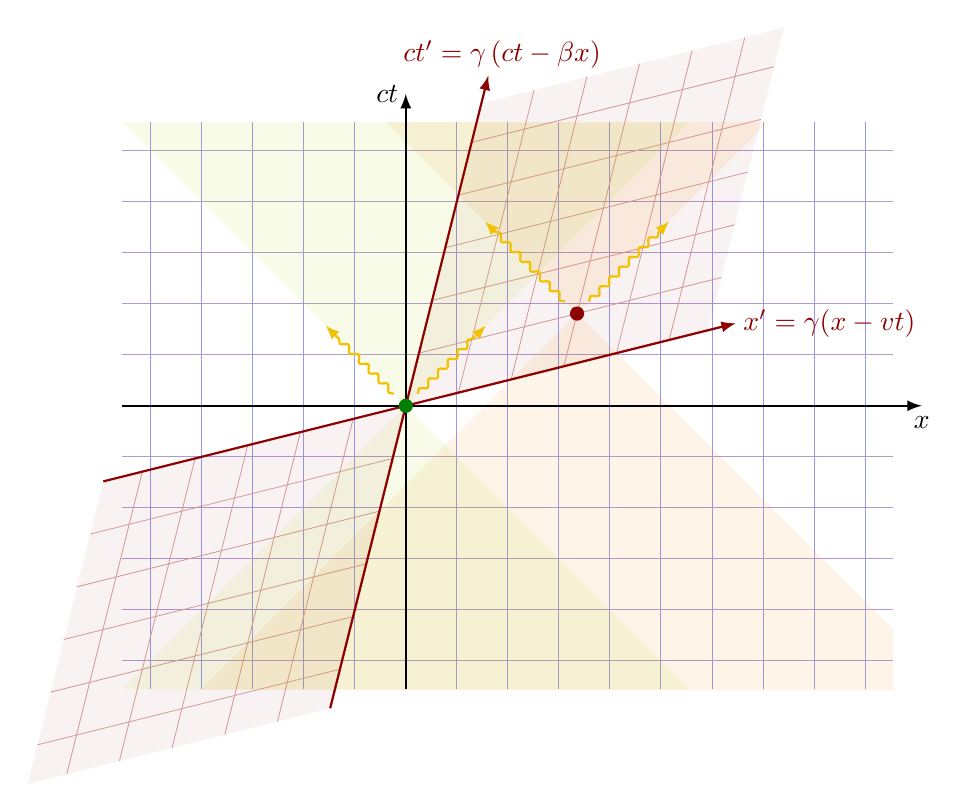
\begin{tikzpicture}[scale=1.8]
  \message{Lorentz boost^^J}
  
  \def\xmax{2}
  \def\xmaxp{2.2} % maximum of rotated axis
  \def\ext{4*\d} % extension x axis
  \def\Nlines{5} % number of world lines (at constant x/t)
  \pgfmathsetmacro\ang{atan(1/4)} % angle between x and x' axes
  \pgfmathsetmacro\d{0.9*\xmax/\Nlines} % grid size
  \pgfmathsetmacro\D{\d/cos(\ang)/sqrt(1-tan(\ang)^2)} % grid size, boosted
  \coordinate (O) at (0,0);
  \coordinate (X) at (\xmax+\ext+0.2,0);
  \coordinate (T) at (0,\xmax+0.2);
  \coordinate (X') at (\ang:\xmaxp+0.2);
  \coordinate (T') at (90-\ang:\xmaxp+0.2);
  \coordinate (B) at ($(\ang:3*\D)+(90-\ang:1*\D)$); % event
  
  % WORLD LINE GRID
  \message{  Making world lines...^^J}
  \foreach \i [evaluate={\x=\i*\d;}] in {1,...,\Nlines}{
    \message{  Running i/N=\i/\Nlines, x=\x...^^J}
    \draw[world line]   (-\x,-\xmax) -- (-\x,\xmax);
    \draw[world line]   ( \x,-\xmax) -- ( \x,\xmax);
    \draw[world line t] (-\xmax,-\x) -- (\xmax+\ext,-\x);
    \draw[world line t] (-\xmax, \x) -- (\xmax+\ext, \x);
  }
  \foreach \i [evaluate={\x=(\Nlines+\i)*\d;}] in {1,...,4}{
    \message{  Running i/N=\i/\Nlines, x=\x...^^J}
    \draw[world line] (\x,-\xmax) -- ( \x,\xmax);
  }
  
  % BOOSTED WORLD LINE GRID
  \message{  Making world lines for boosted frame...^^J}
  \fill[mydarkred,opacity=0.05]
    (O) --++ (\ang:\xmaxp) --++ (90-\ang:\xmaxp) --++ (\ang:-\xmaxp) -- cycle;
  \fill[mydarkred,opacity=0.05]
    (O) --++ (\ang:-\xmaxp) --++ (90-\ang:-\xmaxp) --++ (\ang:\xmaxp) -- cycle;
  \foreach \i [evaluate={\x=\i*\D;}] in {1,...,\Nlines}{
    \message{  Running i/N=\i/\Nlines, x=\x...^^J}
    \draw[world line'] (\ang:-\x) --++ (90-\ang:-\xmaxp);
    \draw[world line'] (90-\ang:-\x) --++ (\ang:-\xmaxp);
    \draw[world line'] (\ang:\x) --++ (90-\ang:\xmaxp);
    \draw[world line'] (90-\ang:\x) --++ (\ang:\xmaxp);
  }
  
  % LIGHT CONES
  \begin{scope}
    \clip (-\xmax,-\xmax) rectangle (\xmax+\ext,\xmax);
    \fill[myorange!70!red,opacity=0.09,shift={(B)}]
      (0,0) -- (\xmax,\xmax) -- (-\xmax,\xmax) -- (2*\xmax,-2*\xmax) -- (-2*\xmax,-2*\xmax) -- cycle;
  \end{scope}
  \fill[myorange!70!green,opacity=0.09]
    (O) -- (\xmax,\xmax) -- (-\xmax,\xmax) -- (\xmax,-\xmax) -- (-\xmax,-\xmax) -- cycle;
  
  % PHOTONS
  \draw[photon] (135:0.12) -- (135:0.4*\xmax);
  \draw[photon] (45:0.12) -- (45:0.4*\xmax);
  \draw[photon] (B)++(135:0.12) --++ (135:0.4*\xmax);
  \draw[photon] (B)++(45:0.12) --++ (45:0.4*\xmax);
  
  % AXES
  \draw[->,thick] (0,-\xmax) -- (T) node[left=-1] {$ct$};
  \draw[->,thick] (-\xmax,0) -- (X) node[below=0] {$x$};
  \draw[->,thick,mydarkred] (90-\ang:-\xmaxp) -- (T')
    node[right=5,above=-1] {$ct' = \gamma\left(ct-\beta x\right)$};
  \draw[->,thick,mydarkred] (\ang:-\xmaxp) -- (X') node[right=-1] {$x' = \gamma(x-vt)$};
  
  % EVENTS
  \fill[mydarkgreen] (O) circle(0.05); % event A
  \fill[mydarkred] (B) circle(0.05); % event B
  
\end{tikzpicture}


% SPACETIME DIAGRAM - EUCLIDEAN ROTATION
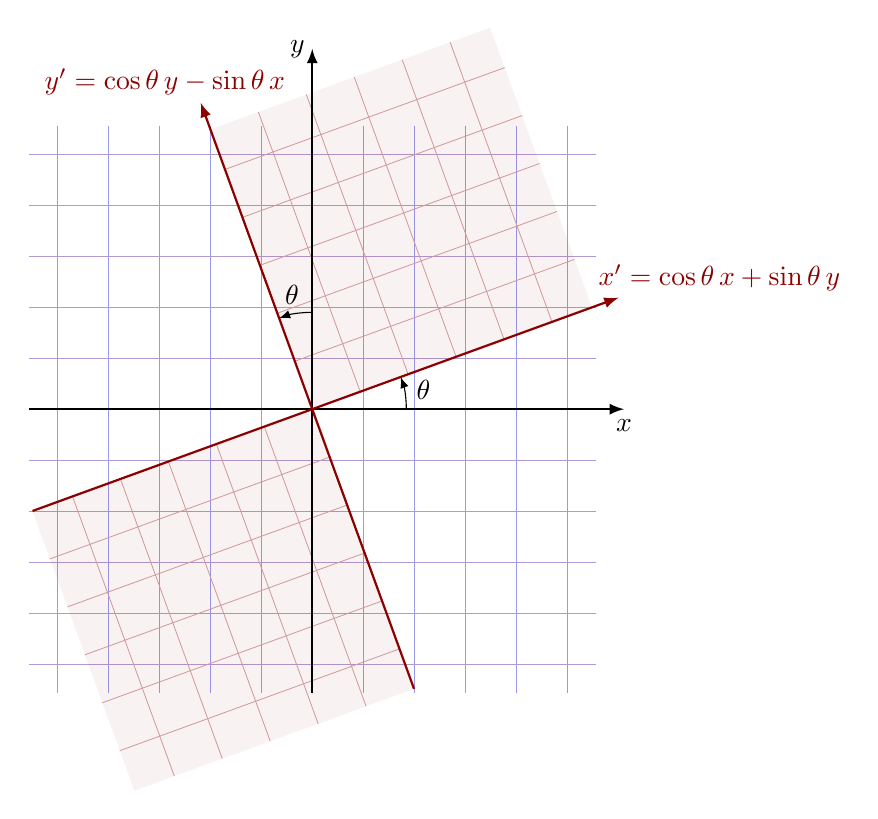
\begin{tikzpicture}[scale=1.8]
  \message{Rotation^^J}
  
  \def\xmax{2}
  \def\xmaxp{2.1} % maximum of rotated axis
  \def\Nlines{5} % number of world lines (at constant x/t)
  \pgfmathsetmacro\ang{20} % angle between x and x' axes
  \pgfmathsetmacro\d{0.9*\xmax/\Nlines} % grid size
  \coordinate (O) at (0,0);
  \coordinate (X) at (\xmax+0.2,0);
  \coordinate (T) at (0,{(1+0.5*sin(\ang))*\xmax+0.2});
  \coordinate (X') at (\ang:\xmaxp+0.2);
  \coordinate (T') at (90+\ang:\xmaxp+0.2);
  
  % WORLD LINE GRID
  \message{  Making world lines...^^J}
  \foreach \i [evaluate={\x=\i*\d;}] in {1,...,\Nlines}{
    \message{  Running i/N=\i/\Nlines, x=\x...^^J}
    \draw[world line]   (-\x,-\xmax) -- (-\x,\xmax);
    \draw[world line]   ( \x,-\xmax) -- ( \x,\xmax);
    \draw[world line t] (-\xmax,-\x) -- (\xmax,-\x);
    \draw[world line t] (-\xmax, \x) -- (\xmax, \x);
  }
  
  % BOOSTED WORLD LINE GRID
  \message{  Making world lines for boosted frame...^^J}
  \fill[mydarkred,opacity=0.05]
    (O) --++ (\ang:\xmaxp) --++ (90+\ang:\xmaxp) --++ (\ang:-\xmaxp) -- cycle;
  \fill[mydarkred,opacity=0.05]
    (O) --++ (\ang:-\xmaxp) --++ (90+\ang:-\xmaxp) --++ (\ang:\xmaxp) -- cycle;
  \foreach \i [evaluate={\x=\i*\d;}] in {1,...,\Nlines}{
    \message{  Running i/N=\i/\Nlines, x=\x...^^J}
    \draw[world line'] (\ang:-\x) --++ (90+\ang:-\xmaxp);
    \draw[world line'] (90+\ang:-\x) --++ (\ang:-\xmaxp);
    \draw[world line'] (\ang:\x) --++ (90+\ang:\xmaxp);
    \draw[world line'] (90+\ang:\x) --++ (\ang:\xmaxp);
  }
  
  % AXES
  \draw[->,thick] (0,-\xmax) -- (T) node[left=-1] {$y$};
  \draw[->,thick] (-\xmax,0) -- (X) node[below=0] {$x$};
  \draw[->,thick,mydarkred] (90+\ang:-\xmaxp) -- (T')
    node[left=13,above=-1] {$y'=\cos\theta\,y-\sin\theta\,x$};
  \draw[->,thick,mydarkred] (\ang:-\xmaxp) -- (X')
    node[above=7,right=-11] {$x'=\cos\theta\,x+\sin\theta\,y$};
  
  % ANGLES
  \draw pic[->,"$\theta$",draw=black,angle radius=34,angle eccentricity=1.2] {angle = X--O--X'};
  \draw pic[->,"$\theta$",draw=black,angle radius=35,angle eccentricity=1.2] {angle = T--O--T'};
  
\end{tikzpicture}


% SPACETIME DIAGRAM - GALILEAN TRANSFORMATION
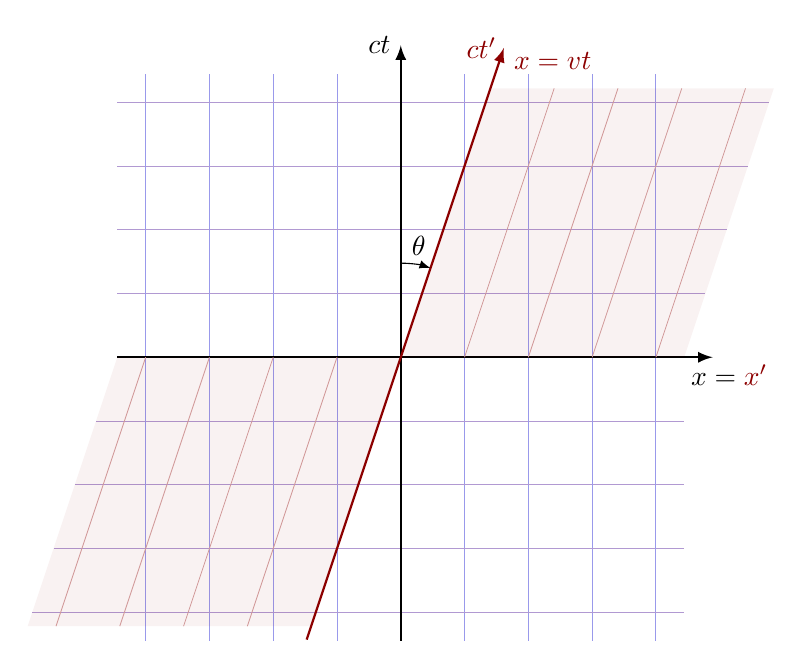
\begin{tikzpicture}[scale=1.8]
  \message{Galilean transformation^^J}
  
  \def\xmax{2}
  \def\xmaxp{2.1} % maximum of rotated axis
  \def\Nlines{4} % number of world lines (at constant x/t)
  \pgfmathsetmacro\d{0.9*\xmax/\Nlines} % grid size
  \pgfmathsetmacro\ang{atan(1/3)} % angle
  \coordinate (O) at (0,0);
  \coordinate (X) at (\xmax+0.2,0);
  \coordinate (T) at (0,\xmax+0.2);
  \coordinate (X') at (\ang:\xmaxp+0.2);
  \coordinate (T') at (90-\ang:\xmaxp+0.2);
  
  % WORLD LINES GRID
  \message{  Making world lines...^^J}
  \foreach \i [evaluate={\x=\i*\d;}] in {1,...,\Nlines}{
    \message{  Running i/N=\i/\Nlines, x=\x...^^J}
    \draw[world line]   (-\x,-\xmax) -- (-\x,\xmax);
    \draw[world line]   ( \x,-\xmax) -- ( \x,\xmax);
    \draw[world line t] ({-\xmax-tan(\ang)*\x},-\x) -- (\xmax,-\x);
    \draw[world line t] (-\xmax,\x) -- ({\xmax+tan(\ang)*\x},\x);
  }
  
  % AXES
  \draw[->,thick] (0,-\xmax) -- (T) node[left=0] {$ct$};
  \draw[->,thick] (-\xmax,0) -- (X) node[right=6,below=-1] {$x={\color{mydarkred}x'}$};
  \draw[->,thick,mydarkred] (90-\ang:-\xmaxp) -- (T')
    node[left=-1] {$ct'$}
    node[right=2,below right=-2] {$x = vt$};
  
  % WORLD LINES GRID - BOOSTED
  \message{  Making world lines, boosted...^^J}
  \fill[mydarkred,opacity=0.05]
    (O) --++ (90-\ang:\xmax) --++ (\xmax,0) --++ (90-\ang:-\xmax) -- cycle;
  \fill[mydarkred,opacity=0.05]
    (O) --++ (90-\ang:-\xmax) --++ (-\xmax,0) --++ (90-\ang:\xmax) -- cycle;
  \foreach \i [evaluate={\x=\i*\d;}] in {1,...,\Nlines}{
    \message{  Running i/N=\i/\Nlines, x=\x...^^J}
    \draw[world line'] (\x,0) --++ (90-\ang:\xmax);
    \draw[world line'] (-\x,0) --++ (90-\ang:-\xmax);
  }
  
  \draw pic[<-,"$\theta$",draw=black,angle radius=34,angle eccentricity=1.2] {angle = T'--O--T};
  
\end{tikzpicture}


% SPACETIME DIAGRAM - LORENTZ BOOST
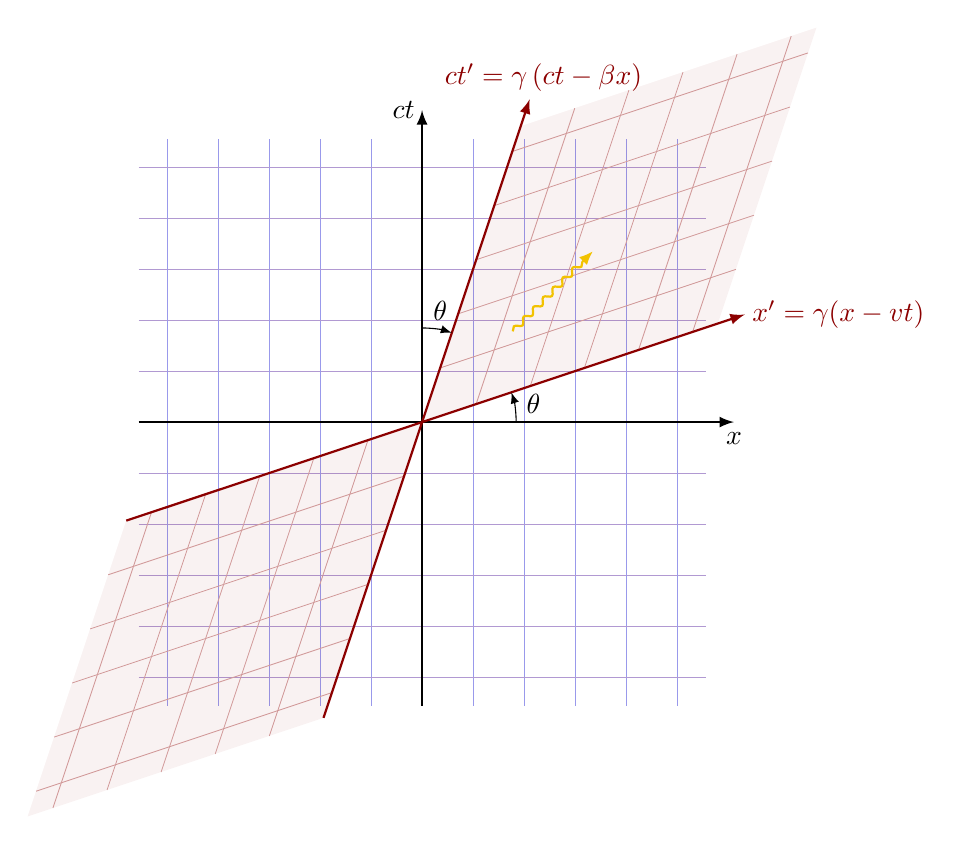
\begin{tikzpicture}[scale=1.8]
  \message{Lorentz boost^^J}
  
  \def\xmax{2}
  \def\xmaxp{2.2} % maximum of rotated axis
  \def\Nlines{5} % number of world lines (at constant x/t)
  \pgfmathsetmacro\ang{atan(1/3)} % angle between x and x' axes
  \pgfmathsetmacro\d{0.9*\xmax/\Nlines} % grid size
  \pgfmathsetmacro\D{\d/cos(\ang)/sqrt(1-tan(\ang)^2)} % grid size, boosted
  \coordinate (O) at (0,0);
  \coordinate (X) at (\xmax+0.2,0);
  \coordinate (T) at (0,\xmax+0.2);
  \coordinate (X') at (\ang:\xmaxp+0.2);
  \coordinate (T') at (90-\ang:\xmaxp+0.2);
  
  % WORLD LINE GRID
  \message{  Making world lines...^^J}
  \foreach \i [evaluate={\x=\i*\d;}] in {1,...,\Nlines}{
    \message{  Running i/N=\i/\Nlines, x=\x...^^J}
    \draw[world line]   (-\x,-\xmax) -- (-\x,\xmax);
    \draw[world line]   ( \x,-\xmax) -- ( \x,\xmax);
    \draw[world line t] (-\xmax,-\x) -- (\xmax,-\x);
    \draw[world line t] (-\xmax, \x) -- (\xmax, \x);
  }
  
  % BOOSTED WORLD LINE GRID
  \message{  Making world lines for boosted frame...^^J}
  \fill[mydarkred,opacity=0.05]
    (O) --++ (\ang:\xmaxp) --++ (90-\ang:\xmaxp) --++ (\ang:-\xmaxp) -- cycle;
  \fill[mydarkred,opacity=0.05]
    (O) --++ (\ang:-\xmaxp) --++ (90-\ang:-\xmaxp) --++ (\ang:\xmaxp) -- cycle;
  \foreach \i [evaluate={\x=\i*\D;}] in {1,...,\Nlines}{
    \message{  Running i/N=\i/\Nlines, x=\x...^^J}
    \draw[world line'] (\ang:-\x) --++ (90-\ang:-\xmaxp);
    \draw[world line'] (90-\ang:-\x) --++ (\ang:-\xmaxp);
    \draw[world line'] (\ang:\x) --++ (90-\ang:\xmaxp);
    \draw[world line'] (90-\ang:\x) --++ (\ang:\xmaxp);
  }
  
  % AXES
  \draw[->,thick] (0,-\xmax) -- (T) node[left=-1] {$ct$};
  \draw[->,thick] (-\xmax,0) -- (X) node[below=0] {$x$};
  \draw[->,thick,mydarkred] (90-\ang:-\xmaxp) -- (T')
    node[right=5,above=-1] {$ct' = \gamma\left(ct-\beta x\right)$};
  \draw[->,thick,mydarkred] (\ang:-\xmaxp) -- (X') node[right=-1] {$x' = \gamma(x-vt)$};
  
  % ANGLES
  \draw pic[->,"$\theta$",draw=black,angle radius=34,angle eccentricity=1.2] {angle = X--O--X'};
  \draw pic[<-,"$\theta$",draw=black,angle radius=34,angle eccentricity=1.2] {angle = T'--O--T};
  
  % PHOTON
  \draw[photon] (0.32*\xmax,0.32*\xmax) --++ (45:0.4*\xmax);
  
\end{tikzpicture}


% SPACETIME DIAGRAM - INVERSE LORENTZ BOOST
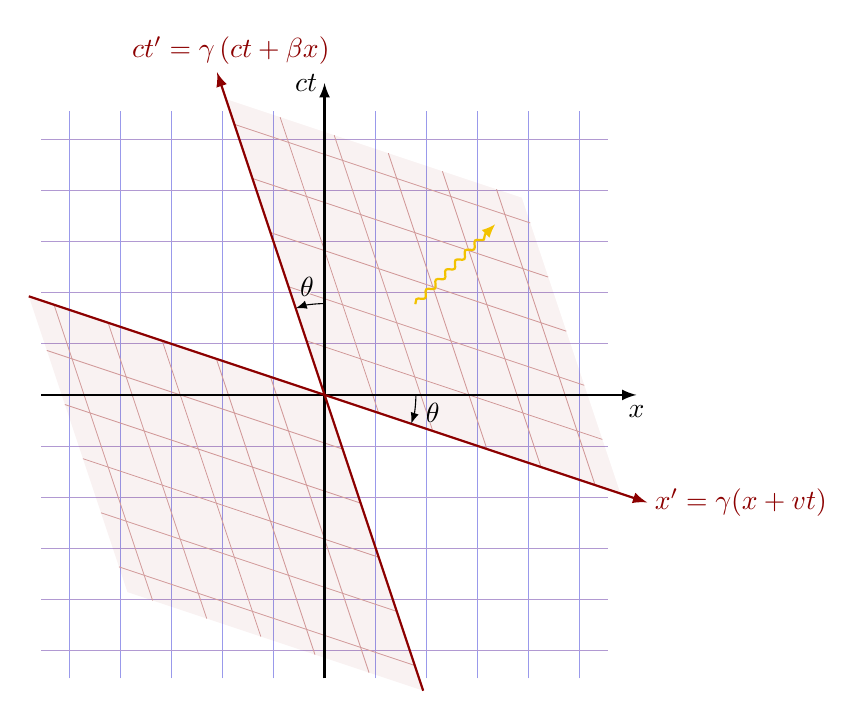
\begin{tikzpicture}[scale=1.8]
  \message{Inverse Lorentz boost^^J}
  
  \def\xmax{2}
  \def\xmaxp{2.2} % maximum of rotated axis
  \def\Nlines{5} % number of world lines (at constant x/t)
  \pgfmathsetmacro\ang{atan(-1/3)} % inverted angle
  \pgfmathsetmacro\d{0.9*\xmax/\Nlines} % grid size
  \pgfmathsetmacro\D{\d/cos(\ang)/sqrt(1-tan(\ang)^2)} % grid size, boosted
  \coordinate (O) at (0,0);
  \coordinate (X) at (\xmax+0.2,0);
  \coordinate (T) at (0,\xmax+0.2);
  \coordinate (X') at (\ang:\xmaxp+0.2);
  \coordinate (T') at (90-\ang:\xmaxp+0.2);
  
  % WORLD LINE GRID
  \message{  Making world lines...^^J}
  \foreach \i [evaluate={\x=\i*\d;}] in {1,...,\Nlines}{
    \message{  Running i/N=\i/\Nlines, x=\x...^^J}
    \draw[world line]   (-\x,-\xmax) -- (-\x,\xmax);
    \draw[world line]   ( \x,-\xmax) -- ( \x,\xmax);
    \draw[world line t] (-\xmax,-\x) -- (\xmax,-\x);
    \draw[world line t] (-\xmax, \x) -- (\xmax, \x);
  }
  
  % BOOSTED WORLD LINE GRID
  \message{  Making world lines for boosted frame...^^J}
  \fill[mydarkred,opacity=0.05]
    (O) --++ (\ang:\xmaxp) --++ (90-\ang:\xmaxp) --++ (\ang:-\xmaxp) -- cycle;
  \fill[mydarkred,opacity=0.05]
    (O) --++ (\ang:-\xmaxp) --++ (90-\ang:-\xmaxp) --++ (\ang:\xmaxp) -- cycle;
  \foreach \i [evaluate={\x=\i*\D;}] in {1,...,\Nlines}{
    \message{  Running i/N=\i/\Nlines, x=\x...^^J}
    \draw[world line'] (\ang:-\x) --++ (90-\ang:-\xmaxp);
    \draw[world line'] (90-\ang:-\x) --++ (\ang:-\xmaxp);
    \draw[world line'] (\ang:\x) --++ (90-\ang:\xmaxp);
    \draw[world line'] (90-\ang:\x) --++ (\ang:\xmaxp);
  }
  
  % AXES
  \draw[->,thick] (0,-\xmax) -- (T) node[left=-1] {$ct$};
  \draw[->,thick] (-\xmax,0) -- (X) node[below=0] {$x$};
  \draw[->,thick,mydarkred] (90-\ang:-\xmaxp) -- (T')
    node[right=5,above=-1] {$ct' = \gamma\left(ct+\beta x\right)$};
  \draw[->,thick,mydarkred] (\ang:-\xmaxp) -- (X') node[right=-1] {$x' = \gamma(x+vt)$};
  
  % ANGLES
  \draw pic[<-,"\contour{myfieldred}{$\theta$}",draw=black,angle radius=33,angle eccentricity=1.2] {angle = X'--O--X};
  \draw pic[->,"\contour{myfieldred}{$\theta$}",draw=black,angle radius=33,angle eccentricity=1.2] {angle = T--O--T'};
  
  % PHOTON
  \draw[photon] (0.32*\xmax,0.32*\xmax) --++ (45:0.4*\xmax);
  
\end{tikzpicture}


% COMMON AXES
\pgfdeclarelayer{back} % to draw on background
\pgfsetlayers{back,main} % set order
\def\xmin{0.23}
\def\xmax{2}
\def\Nlines{6} % number of world lines (at constant x/t)
\def\DNxp{0}   % difference in number of world lines of x' axis
\def\DNyp{0}   % difference in number of world lines of ct' axis
\def\DNy{0}    % difference in number of world lines of ct axis
\def\ang{20}   % angle between x and x' axes
\def\xplabelang{180} % anchor angle of x' axis label
%\pgfmathsetmacro\ang{atan(0.44)} % angle between x and x' axes
\def\axes{
  \pgfmathsetmacro\d{\xmax/(\Nlines+0.4)} % grid size
  \pgfmathsetmacro\D{\d/cos(\ang)/sqrt(1-tan(\ang)^2)} % grid size, boosted
  \pgfmathsetmacro\ymax{\xmax+\DNy*\d} % maximum of y = ct axis
  \pgfmathsetmacro\xmaxp{(\xmax/\d+\DNxp)*\D} % maximum of x' axis
  \pgfmathsetmacro\ymaxp{(\xmax/\d+\DNyp)*\D} % maximum of y' = ct' axis
  \pgfmathsetmacro\Nylines{\Nlines+\DNy} % number of world lines at constant ct'
  \pgfmathsetmacro\Nxplines{\Nlines+\DNxp} % number of world lines at constant x'
  \pgfmathsetmacro\Nyplines{\Nlines+\DNyp} % number of world lines at constant ct'
  \coordinate (O) at (0,0);
  \coordinate (X) at (\xmax+0.15,0);
  \coordinate (T) at (0,\ymax+0.15);
  \coordinate (X') at (\ang:\xmaxp+0.2);
  \coordinate (T') at (90-\ang:\ymaxp+0.2);
  
  % FILL
  \begin{pgfonlayer}{back} % draw on back
    \fill[myfieldred]
      (\ang:-\xmin) -- (\ang:\xmaxp) --++ (90-\ang:\ymaxp) --++ (\ang:-\xmaxp)
      -- (90-\ang:-\xmin) -- cycle;
  \end{pgfonlayer}
  
  % WORLD LINE GRID
  \message{  Making world lines...^^J}
  \foreach \i [evaluate={\x=\i*\d;}] in {1,...,\Nlines}{
    %\message{  Running i/N=\i/\Nlines, x=\x...^^J}
    \draw[world line]   (\x,0) -- (\x,\ymax);
  }
  \foreach \i [evaluate={\t=\i*\d;}] in {1,...,\Nylines}{
    %\message{  Running i/N=\i/\Nlines, t=\t...^^J}
    \draw[world line t] (0,\t) -- (\xmax,\t);
  }
  
  % BOOSTED WORLD LINE GRID
  \message{  Making world lines for boosted frame...^^J}
  \foreach \i [evaluate={\x=\i*\D;}] in {1,...,\Nxplines}{
    %\message{  Running i/N=\i/\Nlines, x=\x...^^J}
    \draw[world line'] (\ang:\x) --++ (90-\ang:\ymaxp);
  }
  \foreach \i [evaluate={\t=\i*\D;}] in {1,...,\Nyplines}{
    %\message{  Running i/N=\i/\Nlines, t=\t...^^J}
    \draw[world line'] (90-\ang:\t) --++ (\ang:\xmaxp);
  }
  
  % AXES
  \draw[->,thick] (0,-\xmin) -- (T) node[left=-1] {$ct$};
  \draw[->,thick] (-\xmin,0) -- (X) node[below=0] {$x$};
  \draw[->,thick,mydarkred] (90-\ang:-\xmin) -- (T')
    node[right=5,above=-1] {$ct'$};
  \draw[->,thick,mydarkred] (\ang:-\xmin) -- (X')
    node[anchor=\xplabelang,inner sep=2] {$x'$};
}


% SPACETIME DIAGRAM - SIMULTANEITY (in S)
\begin{tikzpicture}[scale=1.8]
  \message{Simultaneity^^J}
  
  % AXES
  \axes
  
  % SETTINGS
  \def\L{0.91*\xmaxp} % length of the dashed lines
  \pgfmathsetmacro\xA{2*\d} % x coordinate of A in S
  \pgfmathsetmacro\yA{4*\d} % x coordinate of A in S
  \pgfmathsetmacro\dx{4*\d} % time difference in S
  \pgfmathsetmacro\xAp{(\xA-tan(\ang)*\yA)/cos(\ang)^2/sqrt(1-tan(\ang)^2)} % x coordinate of A in S'
  \pgfmathsetmacro\dtp{4*\d*sin(\ang)/cos(2*\ang)} % time difference between A and B in S'
  \coordinate (A) at (\xA,\yA);
  \coordinate (B) at (\xA+\dx,\yA);
  \coordinate (A') at ($(A)-(\ang:0.11*\xmaxp)$); % left side of dashed line through A
  \coordinate (B') at ($(A')-(90-\ang:\dtp)$); % left side of dashed line through B
  
  % FILL
  \begin{pgfonlayer}{back} % draw on back
    \fill[mylightred]
      %(A') -- (B') -- ($(B)+(\ang:0.07)$) --++ (90-\ang:\dtp) -- cycle;
      (A)++(\ang:-\xAp) --++ (90-\ang:-\dtp) -- ($(B)+(\ang:0.07)$) --++ (90-\ang:\dtp) -- cycle;
    \draw[mylightblue2,line width=1.8] (0,\yA) -- (B);
  \end{pgfonlayer}
  
  % EVENTS
  %\draw[mygreen,thick] (A) -- (B);
  \draw[mygreen,mydashed,thin]
    (A') --++ (\ang:\L);
  \draw[myblue,mydashed,thin]
    (B') --++ (\ang:\L);
  \fill[mydarkgreen] (A) circle(0.04) % event A
    node[above=0] {\contour{myfieldred}{A}};
  \fill[mydarkblue] (B) circle(0.04) % event B
    node[above left=-1] {\contour{mylightred}{B}};
  
  % ARROW
  \draw[mysmallarr,mydarkred] (B)++(\ang:0.13) --++ (90-\ang:\dtp)
    node[pos=0.55,right=-2] {\contour{myfieldred}{$c\Delta t'$}};
  
\end{tikzpicture}



% SPACETIME DIAGRAM - SIMULTANEITY (in S')
\begin{tikzpicture}[scale=1.8]
  \message{Simultaneity^^J}
  
  % AXES
  \axes
  
  % EVENTS
  \def\L{1.1*\xmaxp}
  \coordinate (A) at (90-\ang:3*\D);
  \coordinate (B) at ($(\ang:5*\D)+(90-\ang:3*\D)$);
  %\draw[mygreen,thick] (A) -- (B);
  \draw[mygreen,mydashed,thin]
    (A)++(-0.23*\xmaxp,0) --++ (\L,0);
  \draw[myblue,mydashed,thin]
    (B)++(-0.964*\xmaxp,0) --++ (\L,0);
  \fill[mydarkgreen] (A) circle(0.04) % event A
    node[anchor=-55,inner sep=3] {\contour{mylightblue2}{A}};
  \fill[mydarkblue] (B) circle(0.04) % event B
    node[above left=-1] {\contour{myfieldred}{B}};
  
  % HIGHLIGHT
  \begin{pgfonlayer}{back} % draw on back
    \fill[mylightblue2]
      ($(O)!(A)!(T)$) rectangle ($(B)+(0.06,0)$);
    \draw[mylightred,line width=1.8] (A) -- (B);
  \end{pgfonlayer}
  
  % ARROW
  \pgfmathsetmacro\dt{5*\D*sin(\ang)} % time difference between A and B in S
  \draw[mysmallarr] (A)++(0.81*\xmaxp,0) --++ (0,\dt)
    node[pos=0.5,right=-2] {$c\Delta t$};
  
\end{tikzpicture}


% SPACETIME DIAGRAM - SIMULTANEITY (different order)
\begin{tikzpicture}[scale=1.8]
  \message{Simultaneity^^J}
  
  % AXES
  \def\ang{19.27} % angle between x and x' axes
  \axes
  
  % SETTINGS
  \pgfmathsetmacro\tA{3*\D*cos(\ang)} % time coordinate of A in S
  \coordinate (A) at (90-\ang:3*\D);
  \coordinate (B) at ($(\ang:5*\D)+(90-\ang:2*\D)$);
  
  % FILL
  \begin{pgfonlayer}{back} % draw on back
    \fill[mylightblue2]
      ($(O)!(A)!(T)$) rectangle ($(B)+(0.07,0)$);
    \fill[mylightred]
      (A) --++ (\ang:5*\D) --++ (90-\ang:-\D) --++ (\ang:-5*\D) -- cycle;
  \end{pgfonlayer}
  
  % EVENTS
  \draw[mygreen,mydashed,thin]
    (A)++(-0.22*\xmaxp,0) --++ (1.08*\xmaxp,0) coordinate(A');
  \draw[myblue,mydashed,thin]
    (B)++(-0.906*\xmaxp,0) --++ (1.08*\xmaxp,0);
  \fill[mydarkgreen] (A) circle(0.04) % event A
    node[anchor=-55,inner sep=3] {\contour{mylightblue2}{A}};
  \fill[mydarkblue] (B) circle(0.04) % event B
    node[above left=-2] {B};
  
  % ARROWS
  \draw[mysmallarr,mydarkred] (B)++(\ang:0.09) --++ (90-\ang:\D)
    node[pos=0.55,right=-2.5] {\contour{myfieldred}{$c\Delta t$}$'>0$};
  \draw[mysmallarr] (B)++(0.1,0) --++ ($(0,\tA)-($(O)!(B)!(0,\xmax)$)$)
    node[pos=0.45,right=-2] {\contour{myfieldred}{$c\Delta$}$t<0$};
  
\end{tikzpicture}


% SPACETIME DIAGRAM - TIME DILATION of space point fixed in S
% Inspiration: http://people.uncw.edu/hermanr/GR/Minkowski/Minkowski.pdf
\begin{tikzpicture}[scale=1.8]
  \message{Time dialation (fixed space point in S)^^J}
  
  % AXES
  \axes
  
  % SETTINGS
  \pgfmathsetmacro\dt{5*\d} % time difference in S
  \pgfmathsetmacro\dtp{\dt*cos(\ang)/cos(2*\ang)} % time difference in S'
  \pgfmathsetmacro\dxp{\dt*sin(\ang)/cos(2*\ang)} % distance in S'
  \pgfmathsetmacro\xBp{(-tan(\ang)*\dt)/cos(\ang)^2/sqrt(1-tan(\ang)^2)} % x coordinate of A in S'
  \coordinate (A) at (0,0);
  \coordinate (B) at (0,\dt);
  \coordinate (C) at ($(B)+(\ang:\dxp)$);
  
  % FILL
  \begin{pgfonlayer}{back} % draw on back
    \fill[mylightred] (A) -- (B) -- (C) -- cycle;
  \end{pgfonlayer}
  
  % TRIANGLE
  \draw[very thick,myred,rounded corners=0.1]
    (A) -- (C) node[midway,right=-2] {\contour{myfieldred}{$c\Delta t'$}}
        -- (B) node[midway,above=0] {\contour{white}{$\Delta x'$}}
        -- cycle node[pos=0.5,left=-2] {$c\Delta t$};
  \fill[mydarkred] (A) circle(0.03) node[above left=0] {A};
  \fill[mydarkred] (B) circle(0.03) node[below=1,left=0] {B};
  \fill[mydarkred] (C) circle(0.03) node[below=0,right=0] {\contour{myfieldred}{B$'$}};
  
\end{tikzpicture}


% SPACETIME DIAGRAM - TIME DILATION of space point fixed in S (alternative derivation)
% Inspiration: http://people.uncw.edu/hermanr/GR/Minkowski/Minkowski.pdf
\begin{tikzpicture}[scale=1.8]
  \message{Time dialation (fixed space point in S)^^J}
  
  % AXES
  \axes
  
  % SETTINGS
  \pgfmathsetmacro\xA{4*\d} % x coordinate of A in S
  \pgfmathsetmacro\yA{3*\d} % x coordinate of A in S
  \pgfmathsetmacro\dt{3*\d} % time difference in S
  \pgfmathsetmacro\dtp{\dt*cos(\ang)/cos(2*\ang)} % time difference in S'
  \pgfmathsetmacro\dxp{\dt*sin(\ang)/cos(2*\ang)} % distance in S'
  \pgfmathsetmacro\xBp{(\xA-tan(\ang)*(\yA+\dt))/cos(\ang)^2/sqrt(1-tan(\ang)^2)} % x coordinate of A in S'
  \coordinate (A) at (\xA,\yA);
  \coordinate (B) at (\xA,\yA+\dt);
  \coordinate (C) at ($(A)-(\ang:\dxp)$);
  
  % FILL
  \begin{pgfonlayer}{back} % draw on back
    \fill[mylightblue2]
      ($(O)!(A)!(T)$) rectangle (B);
    \fill[mylightred]
      (B) -- (C) --++ (\ang:-\xBp) --++ (90-\ang:\dtp) -- cycle;
  \end{pgfonlayer}
  
  % TRIANGLE
  \draw[very thick,myred,rounded corners=0.1]
    (A) -- (C) node[midway,below=0] {\contour{myfieldred}{$\Delta x'$}}
        -- (B) node[midway,left=-2] {\contour{mylightred}{$c\Delta t'$}}
        -- cycle node[pos=0.52,right=-2] {\contour{myfieldred}{$c\Delta t$}};
  \fill[mydarkred] (A) circle(0.03) node[below=0,right=0] {\contour{myfieldred}{A}};
  \fill[mydarkred] (B) circle(0.03) node[below=1,right=0] {\contour{myfieldred}{B}};
  \fill[mydarkred] (C) circle(0.03);
  
\end{tikzpicture}


% SPACETIME DIAGRAM - TIME DILATION of fixed space point fixed in S'
% Inspiration: http://people.uncw.edu/hermanr/GR/Minkowski/Minkowski.pdf
\begin{tikzpicture}[scale=1.8]
  \message{Time dialation (fixed space point in S')^^J}
  
  % AXES
  \axes
  
  % SETTINGS
  \pgfmathsetmacro\xAp{2*\D} % x coordinate of A in S'
  \pgfmathsetmacro\yAp{2*\D} % x coordinate of A in S'
  \pgfmathsetmacro\dtp{3*\D} % time difference in S'
  \pgfmathsetmacro\dx{\dtp*sin(\ang)} % distance in S'
  \coordinate (A) at ($(\ang:\xAp)+(90-\ang:\yAp)$);
  \coordinate (B) at ($(A)+(90-\ang:\dtp)$);
  \coordinate (C) at ($(A)+(\dx,0)$);
  
  % FILL
  \begin{pgfonlayer}{back} % draw on back
    \fill[mylightblue2]
      ($(O)!(A)!(T)$) rectangle (B);
    \fill[mylightred]
      (A) --++ (\ang:-\xAp) --++ (90-\ang:\dtp) -- (B) -- cycle;
  \end{pgfonlayer}
  
  % TRIANGLE
  \draw[very thick,myred,rounded corners=0.1]
    (A) -- (C) node[midway,below=-1] {\contour{myfieldred}{$\Delta x'$}}
        -- (B) node[midway,right=-2] {\contour{myfieldred}{$c\Delta t$}}
        -- cycle node[pos=0.52,left=-2] {\contour{mylightred}{$c\Delta t'$}};
  \fill[mydarkred] (A) circle(0.03) node[below=2,left=-2] {\contour{myfieldred}{A}};
  \fill[mydarkred] (B) circle(0.03) node[above=1,left=-1] {\contour{myfieldred}{B}};
  \fill[mydarkred] (C) circle(0.03);
  
\end{tikzpicture}


% SPACETIME DIAGRAM - LENGTH CONTRACTION of rod at rest in S
% Inspiration: http://people.uncw.edu/hermanr/GR/Minkowski/Minkowski.pdf
\def\ang{23} % angle between x and x' axes
\begin{tikzpicture}[scale=1.8]
  \message{Length contraction (rod at rest in S)^^J}
  
  % AXES
  \def\Nlines{7} % number of world lines (at constant x/t)
  \axes
  
  % SETTINGS
  \pgfmathsetmacro\xA{2*\d} % triangle left corner x coordinate in S
  \pgfmathsetmacro\yA{4*\d} % triangle left corner y=ct coordinate in S
  \pgfmathsetmacro\Lz{4*\d} % proper/rest length L0 in S
  \pgfmathsetmacro\L{\Lz/cos(\ang)} % length L in S'
  \coordinate (L) at (\Lz,0); % rod end in S
  \coordinate (L') at (\ang:\L); % rod end in S'
  \coordinate (A) at (\xA,\yA); % point A in triangle
  \coordinate (B) at (\xA+\Lz,\yA); % point B in triangle
  \coordinate (B') at (\xA+\Lz,{\yA+\Lz*tan(\ang)}); % point B' in triangle
  
  % FILL
  \begin{pgfonlayer}{back} % draw on back
    \fill[mylightblue2] (\xA,-\xmin) rectangle (\xA+\Lz,\xmax);
  \end{pgfonlayer}
  \draw[->,thick,mydarkbrown] (\xA,-\xmin) --++ (0,\xmin+\xmax+0.2);
  \draw[->,thick,mydarkbrown] (\xA+\Lz,-\xmin) --++ (0,\xmin+\xmax+0.2);
  
  % ROD
  \draw[rod] (\xA,0) --++ (L)
    node[midway,below=-1] {$L_0$};
  \draw[rod] (\ang:{\xA/cos(\ang)}) --++ (L')
    node[pos=0.485,above=1] {\contour{mylightblue2}{$L$}};
  
  % TRIANGLE
  \draw[very thick,myred,rounded corners=0.1]
    (A) -- (B') node[midway,above=0] {\contour{mylightblue2}{$\Delta x'$}}
        -- (B) node[midway,right=-2] {\contour{myfieldred}{$c\Delta t$}}
        -- cycle node[pos=0.51,below=-1] {\contour{mylightblue2}{$\Delta x$}};
  %\fill[myfieldred] (A)++(185:0.089) circle(0.04);
  %\fill[mydarkred] (A) circle(0.03) node[below=1,left=-2.7] {A};
  \fill[myfieldred] (A)++(200:0.1) circle(0.04);
  \fill[mydarkred] (A) circle(0.03) node[below=1,left=-2.3] {\contour{myfieldred}{A}};
  \fill[mydarkred] (B) circle(0.03) node[below=1,right=0] {\contour{myfieldred}{B}};
  \fill[mydarkred] (B') circle(0.03) node[above=2,right=-1] {\contour{myfieldred}{B$'$}};
  
\end{tikzpicture}


% SPACETIME DIAGRAM - LENGTH CONTRACTION of moving rod (at rest in S')
\begin{tikzpicture}[scale=1.8]
  \message{Length contraction (rod at rest in S')^^J}
  
  % AXES
  \def\Nlines{6} % number of world lines (at constant x/t)
  \axes
  
  % SETTINGS
  \pgfmathsetmacro\Lz{4*\D} % proper/rest length L0 in S'
  \pgfmathsetmacro\L{cos(2*\ang)/cos(\ang)*\Lz} % contracted length L in S
  \coordinate (L) at (\L,0); % rod end in S
  \coordinate (L') at (\ang:\Lz); % rod end in S'
  \coordinate (A) at (90-\ang:{3*\d/cos(\ang)}); % point A in triangle
  \coordinate (B) at ($(A)+(L)$); % point B' in triangle
  \coordinate (B') at ($(A)+(L')$); % point B in triangle
  
  % FILL
  \begin{pgfonlayer}{back} % draw on back
    \fill[mylightred]
      (90-\ang:-\xmin) -- (90-\ang:\xmaxp) --++ (\ang:\Lz) -- (L) --++ (90-\ang:-\xmin) -- cycle;
  \end{pgfonlayer}
  \draw[->,thick,mydarkbrown] (L)++(90-\ang:-\xmin) -- (L) -- (L') --++ (90-\ang:\xmaxp+0.2);
  
  % ROD
  \draw[rod] (O) -- (L)
    node[midway,below=-1] {$L$};
  \draw[rod] (O) -- (L')
    node[pos=0.49,above=1] {\contour{mylightred}{$L_0$}};
  
  % TRIANGLE
  \draw[very thick,myred,rounded corners=0.1]
    (A) -- (B') node[midway,above=0] {\contour{mylightred}{$\Delta x'$}}
        -- (B) node[midway,right=-2] {\contour{myfieldred}{$c\Delta t'$}}
        -- cycle node[pos=0.525,below=-1] {\contour{mylightred}{$\Delta x$}};
  \fill[mydarkred] (A) circle(0.03) node[below=0,left=0] {\contour{white}{A}};
  \fill[mydarkred] (B) circle(0.03) node[below=1,right=0] {\contour{myfieldred}{B}};
  \fill[mydarkred] (B') circle(0.03) node[below=0.5,right=-1] {\contour{myfieldred}{B$'$}};
  
\end{tikzpicture}


% SPACETIME DIAGRAM - LADDER PARADOX
\begin{tikzpicture}[scale=2.5]
  \message{Ladder paradox^^J}
  %\def\R{2*\xmax} % radius of clip
  %\clip (-\xmin,\R) |- (\R,-\xmin) arc(0:90:\xmin+\R);
  
  % AXES
  \def\xmin{0.2}
  \def\xmax{2.6}
  \def\ang{33.5}  % angle between x and x' axes
  \def\Nlines{12} % number of world lines (at constant x/t)
  \def\DNy{1}     % difference in number of world lines of y axis (lengthen)
  \def\DNxp{-6}   % difference in number of world lines of x' axis (shorten)
  \def\DNyp{-2}   % difference in number of world lines of y' axis (shorten)
  \def\xplabelang{170} % anchor angle of x' axis label
  \axes
  
  % SETTINGS
  \pgfmathsetmacro\Lz{4*\D} % proper/rest length L0 of ladder in S'
  \pgfmathsetmacro\L{cos(2*\ang)/cos(\ang)*\Lz} % contracted length L in S
  \pgfmathsetmacro\yminb{-0.7*\xmin} % ymin of barn in S
  \pgfmathsetmacro\xb{4.96*\d} % x coordinate of barn in S
  \pgfmathsetmacro\wb{3.08*\d} % width of barn in S
  \pgfmathsetmacro\yA{(\xb+0.04*\d)/tan(\ang)} % y = ct coordinate when ladder is fully in barn in S
  \coordinate (L) at (\L,0); % ladder end in S
  \coordinate (L') at (\ang:\Lz); % ladder end in S'
  \coordinate (A) at (90-\ang:{(\xb+0.04*\d)/sin(\ang)}); % left end of ladder when fully in barn
  \coordinate (B) at ($(A)+(\L,0)$); % right end of ladder when fully in barn
  \coordinate (C) at (90-\ang:{(\xb+\wb+0.08*\d)/sin(\ang)}); % left end of ladder when fully passed through barn
  
  % FILL
  \begin{pgfonlayer}{back} % draw on back (behind axes)
    \fill[mydarkblue!22] % barn frame
      (\xb,\yminb) rectangle (\xb+\wb,\ymax);
    \fill[mylightred] % ladder frame
      (90-\ang:-\xmin) -- (90-\ang:\ymaxp) --++ (\ang:\Lz) -- (L) --++ (90-\ang:-\xmin) -- cycle;
    \begin{scope}
      \clip (0,0) rectangle(1.3*\xmax,\ymax+0.2);
      \draw[myredhighlight,line width=3.1] % highlight simultaneity in S'
        (A)++(\ang:{-\xb/cos(\ang)-0.05}) --++ (\ang:\xmax+3.6*\D)
        (B)++(\ang:{-\xb/cos(\ang)-0.05-\Lz}) --++ (\ang:\xmax+3.8*\D);
      \draw[mypurplehighlight,line width=3.1] % highlight simultaneity in S
        (0,\yA) --++ (\xmax+0.8*\d,0);
    \end{scope}
  \end{pgfonlayer}
  \draw[->,thick,mydarkblue] % barn left door
    (\xb,\yminb) -- (\xb,\ymax+0.15);
  \draw[->,thick,mydarkblue] % barn right door
    (\xb+\wb,\yminb) -- (\xb+\wb,\ymax+0.15);
  \draw[->,thick,mydarkbrown] % rod left end
    (L)++(90-\ang:-\xmin) -- (L) -- (L') --++ (90-\ang:\ymaxp+0.2);
  
  % LADDER
  \draw[rod] (O) -- (L')
    node[pos=0.55,above=2,scale=0.8] {\contour{mylightred}{$L_0$}};
  \draw[rod] (O) -- (L)
    node[pos=0.46,below=1,scale=0.8] {$L$};
  
  % LADDER IN BARN
  \draw[rod] (A) --++ (L');
  \draw[rod] (B) --++ (\ang:-\Lz);
  \draw[rod] (A) --++ (L);
  
  % LADDER RIGHT OF BARN
  \draw[rod] (C) --++ (L');
  \draw[rod] (C) --++ (L);
  
  % LABELS
  \node[mydarkblue,below=0,align=center,scale=0.8,yshift=1] at (\xb+\wb/2,0)
    {barn\\$L<w<L_0$};
  \node[mydarkpurple,right,align=left,scale=0.65,yshift=1.2] at (\xb+3.6*\d,\yA)
    {both doors closed in S};
    %{both doors\\[-3]close in S};
  \node[mydarkred,right,scale=0.65,yshift=1.8,rotate=\ang] at ($(A)+(\ang:\Lz+0.8*\D)$)
    {left door closed in S$'$};
  \node[mydarkred,right,scale=0.65,yshift=0.7,rotate=\ang] at ($(B)+(\ang:0.8*\D)$)
    {right door closed in S$'$};
  
\end{tikzpicture}


% SPACETIME DIAGRAM - LADDER PARADOX from perspective of S' (i.e. in the S' frame)
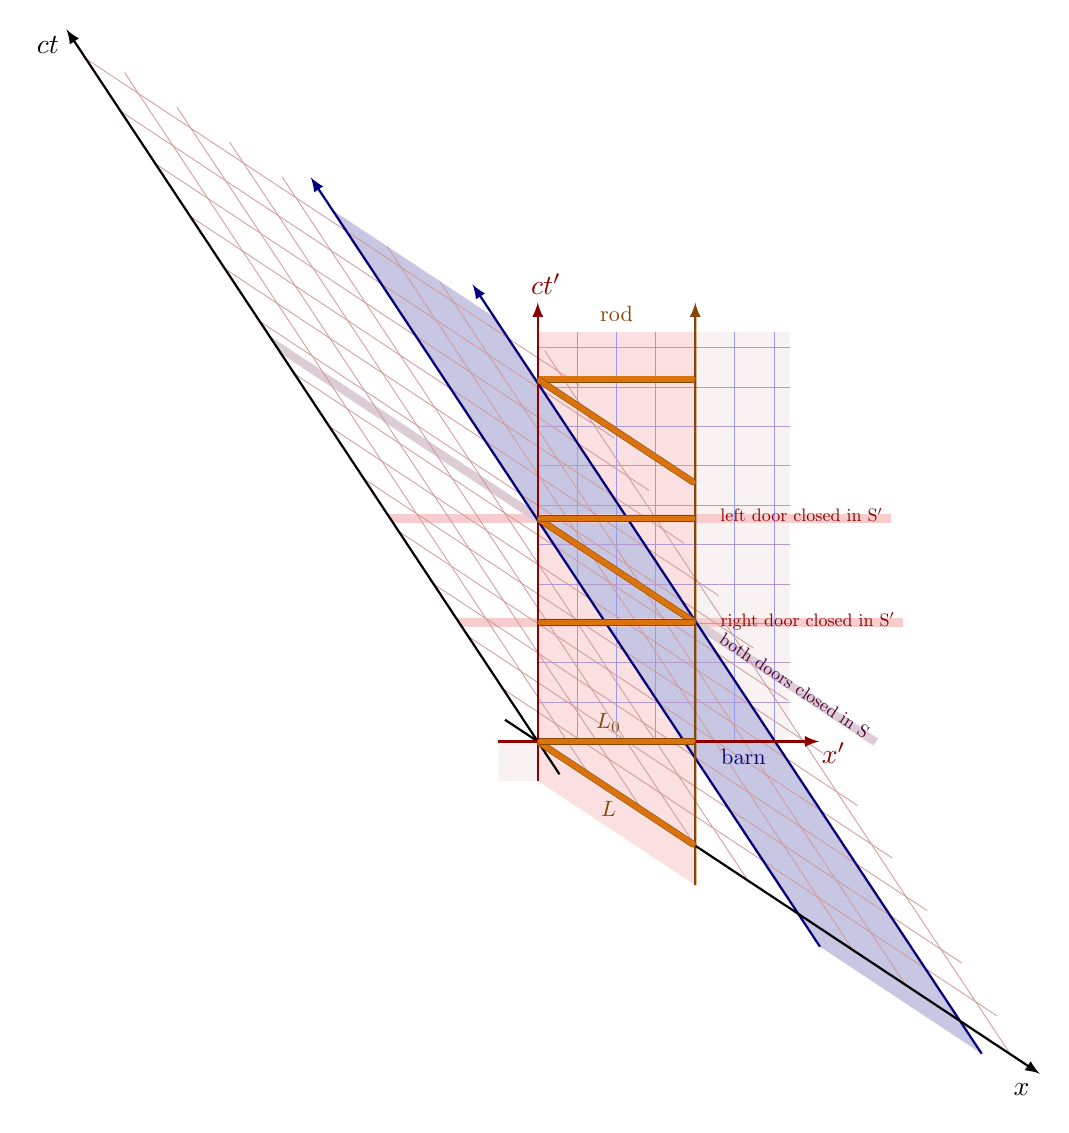
\begin{tikzpicture}[scale=2.5]
  \message{Ladder paradox from the perspective of S'^^J}
  
  % SETTINGS
  \def\ang{-33.5}   % angle between x and x' axes
  \def\Nxlines{9}   % number of world lines (at constant x)
  \def\Nylines{13}  % number of world lines (at constant t)
  \def\Nxplines{6}  % number of world lines (at constant x')
  \def\Nyplines{10} % number of world lines (at constant t')
  \def\xmin{0.2}
  \pgfmathsetmacro\D{2.6/13} % grid size
  \pgfmathsetmacro\d{\D/cos(\ang)/sqrt(1-tan(\ang)^2)} % grid size, boosted
  \pgfmathsetmacro\xmax{(\Nxlines+0.4)*\d}   % maximum of x axis in S
  \pgfmathsetmacro\ymax{(\Nylines+0.4)*\d}   % maximum of y = ct axis in S
  \pgfmathsetmacro\xmaxp{(\Nxplines+0.4)*\D} % maximum of x' axis in S'
  \pgfmathsetmacro\ymaxp{(\Nyplines+0.4)*\D} % maximum of y' = ct' axis in S'
  \pgfmathsetmacro\Lz{4*\D} % proper/rest length L0 of ladder in S'
  \pgfmathsetmacro\L{\Lz/cos(\ang)} % contracted length L in S
  \pgfmathsetmacro\xb{4.96*\d} % x coordinate of barn in S
  \pgfmathsetmacro\wb{3.08*\d} % width of barn in S
  \pgfmathsetmacro\yAp{(\xb+0.04*\d)*sin(\ang)*(1-cot(\ang)^2)} % y' = ct' coordinate when ladder is fully in barn in S
  \pgfmathsetmacro\yBp{\yAp+\L*sin(\ang)} % y' = ct' coordinate when ladder is fully in barn in S
  \coordinate (O) at (0,0);
  \coordinate (X) at (\ang:\xmax+0.05);
  \coordinate (T) at (90-\ang:\ymax+0.05);
  \coordinate (X') at (\xmaxp+0.15,0);
  \coordinate (T') at (0,\ymaxp+0.15);
  \coordinate (L) at (\ang:\L); % ladder end in S
  \coordinate (L') at (\Lz,0); % ladder end in S'
  \coordinate (A) at (0,\yAp); % left end of ladder when fully in barn in S
  \coordinate (B) at ($(A)+(L)$); % right end of ladder when fully in barn in S
  \coordinate (C) at (0,{(\xb+\wb+0.08*\d)*sin(\ang)*(1-cot(\ang)^2)}); % left end of ladder when fully passed through barn
  
  % FILL
  \fill[myfieldred]
    (-\xmin,0) -| (\xmaxp,\ymaxp) -| (0,-\xmin) -| cycle;
  \fill[mylightred] % ladder frame
    (0,-\xmin) |- (\Lz,\ymaxp) -- ($(L)+(0,-\xmin)$) -- cycle;
  \fill[mydarkblue!22] % barn frame
    (\ang:\xb)++(90-\ang:-\xmin) --++ (90-\ang:\xmin+\ymax)
    --++ (\ang:\wb) --++ (90-\ang:-\xmin-\ymax) -- cycle;
  
  % HIGHLIGHT DOORS OPEN/CLOSED
  \begin{scope}
    \clip (0,0) --++ (90-\ang:\ymax) -- (\xmaxp+1.8*\d,\ymaxp) --++ (0,-1.1*\ymaxp) -- cycle;
    \draw[myredhighlight,line width=3.1] % highlight simultaneity in S'
      ({\yAp*tan(\ang)-0.1},\yAp) -- (\xmaxp+1.6*\d,\yAp)
      ({\yBp*tan(\ang)-0.1},\yBp) -- (\xmaxp+1.8*\d,\yBp);
    \draw[mypurplehighlight,line width=3.1] % highlight simultaneity in S
      (A)++(\ang:-\xb-0.1) --++ (\ang:{\xb+\L+3.75*\d});
  \end{scope}
  
  % BOOSTED WORLD LINE GRID
  \message{  Making world lines for boosted frame...^^J}
  \foreach \i [evaluate={\x=\i*\D;}] in {1,...,\Nxplines}{
    \draw[world line]   (\x,0) -- (\x,\ymaxp);
  }
  \foreach \i [evaluate={\t=\i*\D;}] in {1,...,\Nyplines}{
    \draw[world line t] (0,\t) -- (\xmaxp,\t);
  }
  
  % WORLD LINE GRID
  \message{  Making world lines...^^J}
  \foreach \i [evaluate={\x=\i*\d;}] in {1,...,\Nxlines}{
    \draw[world line'] (\ang:\x) --++ (90-\ang:\ymax);
  }
  \foreach \i [evaluate={\t=\i*\d;}] in {1,...,\Nylines}{
    \draw[world line'] (90-\ang:\t) --++ (\ang:\xmax);
  }
  
  % WORLD LINES BARN & ROD
  \draw[->,thick,mydarkblue] % barn left door
    (\ang:\xb+\wb)++(90-\ang:-\xmin) --++ (90-\ang:\xmin+\ymax+0.2);
  \draw[->,thick,mydarkblue] % barn right door
    (\ang:\xb)++(90-\ang:-\xmin) --++ (90-\ang:\xmin+\ymax+0.2);
  \draw[->,thick,mydarkbrown] % rod right end
    (L)++(0,-\xmin) -- (\Lz,\ymaxp+0.15);
  
  % AXES
  \draw[->,thick] (90-\ang:-\xmin) -- (T) node[below left=-1] {$ct$};
  \draw[->,thick] (\ang:-\xmin) -- (X) node[below left=0] {$x$};
  \draw[->,thick,mydarkred] (0,-\xmin) -- (T')
    node[right=3,above=-1] {$ct'$};
  \draw[->,thick,mydarkred] (-\xmin,0) -- (X')
    node[anchor=140,inner sep=0.5] {$x'$};
  
  % LADDER
  \draw[rod] (O) -- (L)
    node[pos=0.45,below=2,scale=0.8] {$L$};
  \draw[rod] (O) -- (L')
    node[pos=0.45,above=0.6,scale=0.8] {\contour{mylightred}{$L_0$}};
  \draw[rod] (O) -- (L');
  
  % LADDER IN BARN
  \draw[rod] (A) --++ (L);
  \draw[rod] (A) --++ (L');
  \draw[rod] (B) --++ (-\Lz,0);
  
  % LADDER RIGHT OF BARN
  \draw[rod] (C) --++ (L');
  \draw[rod] (C) --++ (L);r
  
  % LABELS
  \node[mydarkbrown,above=1,scale=0.8] at (\Lz/2,\ymaxp)
    {rod};
  \node[mydarkblue,below=0,scale=0.8]
    at ({(\xb+\wb/2)*cos(\ang)*(1-tan(\ang)^2)+0.07},0)
    {\contour{mydarkblue!22}{barn}};
  %\node[mydarkblue,anchor=90-\ang,inner sep=2,scale=0.8,rotate=\ang] at (\ang:\xb+\L/2)
  %  {barn}; %{barn\\$L<w<L_0$};
  \node[mydarkpurple,right,align=left,scale=0.65,yshift=1.6,rotate=\ang]
    at ($(B)+(\ang:0.4*\d)$) {both doors closed in S};
  \node[mydarkred,right,scale=0.65,yshift=1.8] at ($(A)+(\Lz+0.3*\d,0)$)
    {left door closed in S$'$};
  \node[mydarkred,right,scale=0.65,yshift=0.7] at ($(B)+(0.3*\d,0)$)
    {right door closed in S$'$};
  
\end{tikzpicture}


% SPACETIME DIAGRAM of TWIN PARADOX
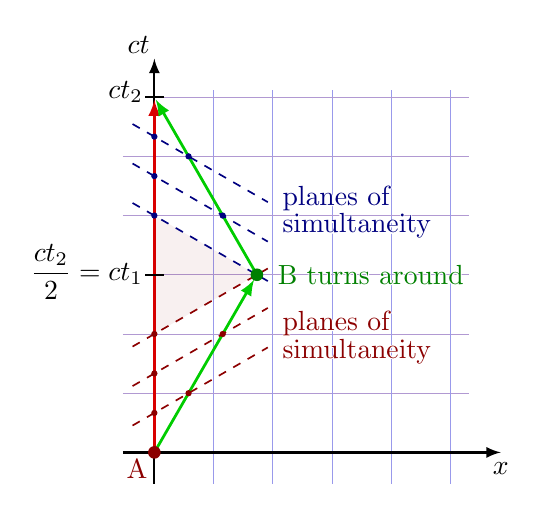
\begin{tikzpicture}[scale=2.0]
  \message{Twin paradox^^J}
  
  \def\xmin{0.2}
  \def\xmax{2}
  \def\ymax{2.3}
  \def\Nlines{5} % number of world lines (at constant x/t)
  \def\ang{60} % angle between ct and ct' axes
  \pgfmathsetmacro\d{0.94*\xmax/\Nlines} % grid size
  \pgfmathsetmacro\dt{3*\d} % time of half trip
  \pgfmathsetmacro\D{\dt/tan(\ang)} % distance between observers
  \pgfmathsetmacro\h{\dt-\D/tan(\ang)} % half time gap of return
  \coordinate (A) at (0,0); % observer A at t=0
  \coordinate (B) at (\D,0); % observer B at t=0
  \coordinate (C) at (\D,\dt); % point of return
  \coordinate (T1) at (0,\dt); % time of return
  \coordinate (T2) at (0,2*\dt); % time of arrival
  
  % WORLD LINES GRID
  \message{  Making world lines...^^J}
  \foreach \i [evaluate={\x=\i*\d;}] in {1,...,\Nlines}{
    \message{  Running i/N=\i/\Nlines, x=\x...^^J}
    \draw[world line]   ( \x,-\xmin) -- ( \x,\ymax);
    \draw[world line t] (-\xmin, \x) -- (\xmax, \x);
  }
  \draw[world line t] (-\xmin,{(\Nlines+1)*\d}) -- (\xmax,{(\Nlines+1)*\d});
  
  % AXES
  \draw[->,thick] (0,-\xmin) -- (0,\ymax+0.2) node[above left=-2] {$ct$};
  \draw[->,thick] (-\xmin,0) -- (\xmax+0.2,0) node[below=0] {$x$};
  
  % VECTORS
  \draw[vector,myred,shorten >=1] (A) -- (T2);
  \draw[vector,mygreen,shorten >=2] (A) -- (C);
  \draw[vector,mygreen,shorten >=1] (C) -- (T2);
  
  % PLANES OF SIMULTANEITY
  \fill[mydarkred,opacity=0.06]
    (0,\h) -- (C) -- (0,2*\dt-\h) -- cycle;
  \pgfmathsetmacro\ystep{\h/3}
  \foreach \i [evaluate={\dy=(\i-1)*\ystep; \ya=\i*\ystep; \yb=2*\dt-\i*\ystep;}] in {1,...,3}{
    \draw[mydarkred,dashed,line width=0.6]
      (0,\ya)++(90-\ang:-0.8*\xmin) --++ (90-\ang:{1.2*\xmin+\D/sin(\ang)});
    \draw[mydarkblue,dashed,line width=0.6]
      (0,\yb)++(\ang-90:-0.8*\xmin) --++ (\ang-90:{1.2*\xmin+\D/sin(\ang)});
    \fill[mydarkred]  (0,\ya) circle(0.02);
    \fill[mydarkblue] (0,\yb) circle(0.02);
    %\fill[mydarkblue] ({\D-\dy*cot(\ang)},\dt+\dy) circle(0.02);
    %\fill[mydarkred]  ({\D-\dy*cot(\ang)},\dt-\dy) circle(0.02);
    \fill[mydarkblue] (C)++(-\ang:{\dy*sin(\ang)/cos(2*\ang)}) circle(0.02);
    \fill[mydarkred]  (C)++( \ang:{\dy*sin(\ang)/cos(2*\ang)}) circle(0.02);
  }
  \fill[mydarkred] (A) circle(0.04) node[below left=-1] {A}; % observer A
  \fill[mydarkgreen] (C) circle(0.04)
    node[right=4] {\contour{white}{B turns around}}; % observer B returns
  \node[mydarkblue,above right=0,align=left] at (2*\d,1.15*\dt)
    {\contour{white}{planes of}\\[-2]\contour{white}{simultaneity}};
  \node[mydarkred,below right=0,align=left] at (2*\d,0.85*\dt)
    {\contour{white}{planes of}\\[-2]\contour{white}{simultaneity}};
  
  % TICKS
  \node[fill=white,inner sep=1,above=1,left=3] at (T1) {$\dfrac{ct_2}{2}=ct_1$};
  \node[fill=white,inner sep=1,above=2,left=3] at (T2) {$ct_2$};
  \tick{T1}{0};
  \tick{T2}{0};
  
\end{tikzpicture}


% SPACETIME DIAGRAM - INVARIANT HYPERBOLOIDS
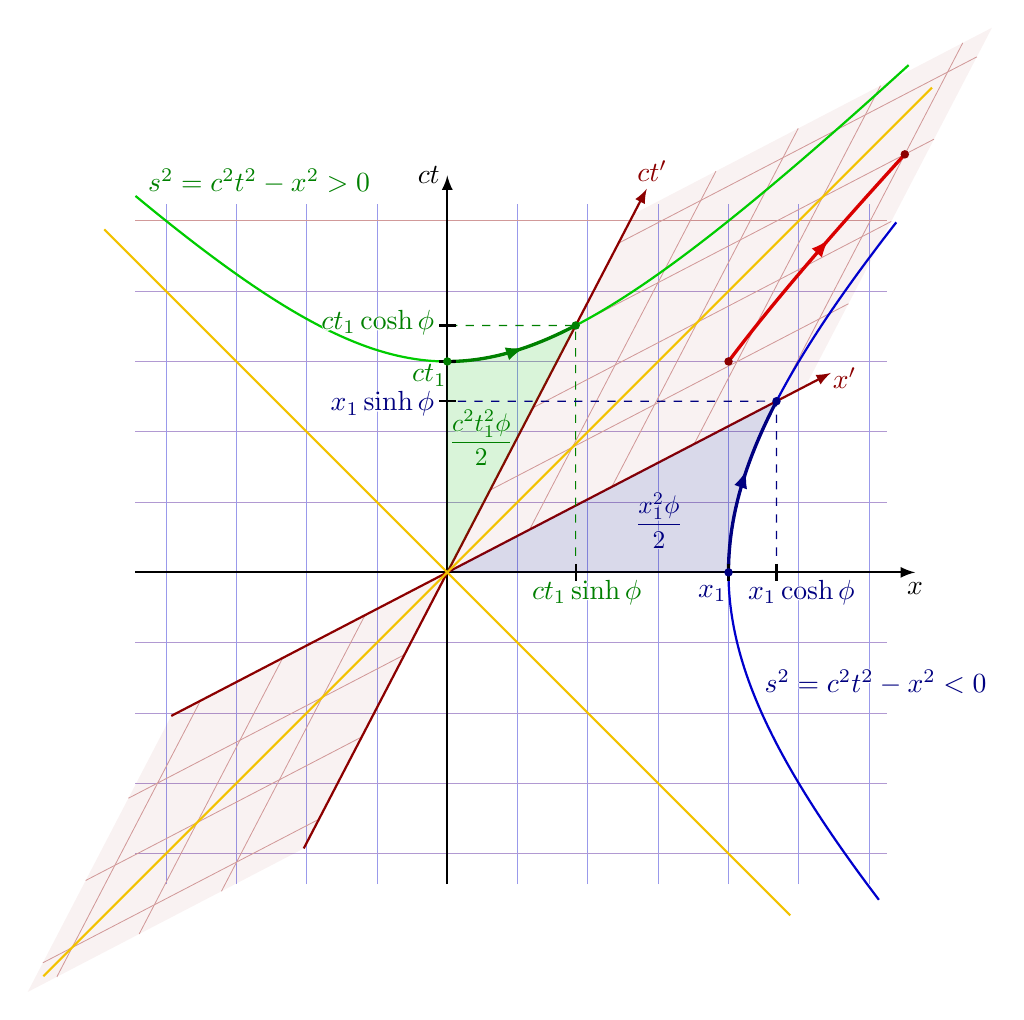
\begin{tikzpicture}[scale=1.8]
  \message{Invariant hyperboloids^^J}
  
  % SETTINGS
  \def\xmin{2.2}
  \def\xmax{3.1}
  \def\ymin{2.2}
  \def\ymax{2.6}
  \def\xmaxp{2.85} % maximum of rotated axis
  \def\Nlines{4} % number of world lines (at constant x/t)
  \pgfmathsetmacro\ang{atan(0.52)} % angle between x and x' axes
  \pgfmathsetmacro\d{0.64*\xmax/\Nlines} % grid size
  \pgfmathsetmacro\D{\d/cos(\ang)/sqrt(1-tan(\ang)^2)} % grid size, boosted
  \pgfmathsetmacro\dextra{(\Nlines+1)*\d} % extra line
  \pgfmathsetmacro\st{3*\d} % spacetime interval
  \pgfmathsetmacro\sx{4*\d} % spacetime interval
  \pgfmathsetmacro\sr{sqrt(\sx^2-\st^2)} % spacetime interval sr^2 = st^2 - sx^2 < 0
  \pgfmathsetmacro\Ax{3*\D*sin(\ang)} % x coordinate of event A
  \pgfmathsetmacro\Ay{3*\D*cos(\ang)} % y coordinate of event A
  \pgfmathsetmacro\Bx{4*\D*cos(\ang)} % x coordinate of event B
  \pgfmathsetmacro\By{4*\D*sin(\ang)} % y coordinate of event B
  \pgfmathsetmacro\Cx{\Ay+\By} % x coordinate of event C' %(\Bx+tan(\ang)*\Ay)/sqrt(1-tan(\ang)^2)
  \coordinate (O)  at (0,0);
  \coordinate (X)  at (\xmax+0.2,0);
  \coordinate (T)  at (0,\ymax+0.2);
  \coordinate (X') at (\ang:\xmaxp+0.2);
  \coordinate (T') at (90-\ang:\xmaxp+0.2);
  \coordinate (A)  at (0,\st);        % event A
  \coordinate (A') at (90-\ang:3*\D); % event A', boosted A
  \coordinate (B)  at (\sx,0);        % event A
  \coordinate (B') at (\ang:4*\D);    % event A', boosted A
  \coordinate (C)  at (4*\d,3*\d);    % event C
  
  % WORLD LINE GRID
  \message{  Making world lines...^^J}
  \foreach \i [evaluate={\x=\i*\d;}] in {1,...,\Nlines}{
    \message{  Running i/N=\i/\Nlines, x=\x...^^J}
    \draw[world line]   (-\x,-\ymin) -- (-\x,\ymax);
    \draw[world line]   ( \x,-\ymin) -- ( \x,\ymax);
    \draw[world line t] (-\xmin,-\x) -- (\xmax,-\x);
    \draw[world line t] (-\xmin, \x) -- (\xmax, \x);
  }
  \draw[world line]    (\dextra,-\ymin)  -- (\dextra,\ymax);
  \draw[world line]    (\dextra+\d,-\ymin) -- (\dextra+\d,\ymax);
  %\draw[world line'] (-\xmin,-\dextra) -- (\xmax,-\dextra);
  \draw[world line'] (-\xmin,\dextra) -- (\xmax,\dextra);
  
  % BOOSTED WORLD LINE GRID
  \message{  Making world lines for boosted frame...^^J}
  \fill[mydarkred,opacity=0.05]
    (O) --++ (\ang:\xmaxp) --++ (90-\ang:\xmaxp) --++ (\ang:-\xmaxp) -- cycle;
  \fill[mydarkred,opacity=0.05]
    (O) --++ (\ang:\D-\xmaxp) --++ (90-\ang:\D-\xmaxp) --++ (\ang:\xmaxp-\D) -- cycle;
  \foreach \i [evaluate={\x=\i*\D;}] in {1,...,\Nlines}{
    \message{  Running i/N=\i/\Nlines, x=\x...^^J};
    \ifnumcomp{\i}{<}{\Nlines}{
      \draw[world line'] (\ang:-\x) --++ (90-\ang:\D-\xmaxp);
      \draw[world line'] (90-\ang:-\x) --++ (\ang:\D-\xmaxp);
    }{}
    \draw[world line'] (\ang:\x) --++ (90-\ang:\xmaxp);
    \draw[world line'] (90-\ang:\x) --++ (\ang:\xmaxp);
  }
  
  % AXES
  \draw[->,thick] (0,-\ymin) -- (T) node[left=-1] {$ct$};
  \draw[->,thick] (-\xmin,0) -- (X) node[below=0] {$x$};
  \draw[->,thick,mydarkred] (90-\ang:\D-\xmaxp) -- (T')
    node[right=2,above=-1] {$ct'$};
  \draw[->,thick,mydarkred] (\ang:\D-\xmaxp) -- (X') node[below=2,right=-3] {$x'$};
  
  % LIGHTCONE
  \draw[myorange,thick]
    (-1.1*\xmin,1.1*\xmin) -- (1.1*\ymin,-1.1*\ymin)
    (-\xmaxp,-\xmaxp) -- (1.2*\xmaxp,1.2*\xmaxp);
  
  % AREA HYPERBOLIC SECTORS
  \fill[mygreen!90!black,opacity=0.15,thick,samples=\Nsamples,smooth,variable=\x,domain=0:\Ax]
    plot(\x,{sqrt((\st)^2+(\x)^2)}) -- (O) -- (A);
  \fill[mydarkblue!90!black,opacity=0.15,thick,samples=\Nsamples,smooth,variable=\y,domain=0:\By]
    plot({sqrt((\sx)^2+(\y)^2)},\y) -- (O) -- (B);
  \node[mydarkgreen,scale=0.92] at (89.5-\ang/2:1.97*\d)
    {\contour{mygreen!90!black!15}{$\dfrac{c^2t_1^2\phi}{2}$}};
  \node[mydarkblue,scale=0.92] at (\ang/2:3.1*\d)
    {\contour{mydarkblue!90!black!15}{$\dfrac{x_1^2\phi}{2}$}};
  
  % SPACELIKE HYPERBOLOIDS
  \draw[mygreen,thick,samples=\Nsamples,smooth,variable=\x,domain=-\xmin:1.05*\xmax]
    plot(\x,{sqrt((\st)^2+(\x)^2)});
  \draw[mydarkgreen,very thick,samples=\Nsamples,variable=\x,domain=0:\Ax,
        decoration={markings,mark=at position 0.58 with {\arrow{latex}}},postaction={decorate}]
    plot(\x,{sqrt((\st)^2+(\x)^2)});
  \node[mydarkgreen,right=1,above right=0] at (-\xmin,\ymax)
    {$s^2 = c^2t^2-x^2>0$};
  
  % TIMELIKE HYPERBOLOIDS
  \draw[myred,very thick,samples=\Nsamples,variable=\y,domain=\st:\Cx,
        decoration={markings,mark=at position 0.58 with {\arrow{latex}}},postaction={decorate}]
    plot({sqrt(\sr^2+(\y)^2)},\y);
  \draw[myblue,thick,samples=\Nsamples,smooth,variable=\y,domain=-1.05*\ymin:0.95*\ymax]
    plot({sqrt(\sx^2+(\y)^2)},\y);
  \draw[mydarkblue,very thick,samples=\Nsamples,variable=\y,domain=0:\By,
        decoration={markings,mark=at position 0.58 with {\arrow{latex}}},postaction={decorate}]
    plot({sqrt(\sx^2+(\y)^2)},\y);
  \node[mydarkblue,right=0] at (0.7*\xmax,-0.25*\xmax)
    {\contour{white}{$s^2 = c^2t^2-x^2<0$}};
  
  % TICKS
  \draw[mydarkgreen,dashed] ({\Ax},0) -- (A') -- (0,{\Ay});
  \draw[mydarkblue,dashed] ({\Bx},0) -- (B') -- (0,{\By});
  \tick{0,\st}{0} node[mydarkgreen,right=4,below left=-2.5] {$ct_1$};
  \tick{\sx,0}{90} node[mydarkblue,below=1,below left=-3] {$x_1$};
  \tick{0,\Ay}{0} node[mydarkgreen,above=1,left=-2]
    {\contour{white}{$ct_1\cosh\phi$}};
  \tick{\Ax,0}{90} node[mydarkgreen,right=4,below=-4]
    {\contour{white}{$ct_1\sinh\phi$}};
  \tick{\Bx,0}{90} node[mydarkblue,right=9,below=-4]
    {\contour{white}{$x_1\cosh\phi$}};
  \tick{0,\By}{0} node[mydarkblue,below=1,left=-2]
    {\contour{white}{$x_1\sinh\phi$}};
  
  % EVENTS
  \fill[mydarkgreen] (A)  circle(0.03); % event A
  \fill[mydarkgreen] (A') circle(0.03); % event A'
  \fill[mydarkblue]  (B)  circle(0.03); % event B
  \fill[mydarkblue]  (B') circle(0.03); % event B'
  \fill[mydarkred]   (C)  circle(0.03); % event C
  \fill[mydarkred] (\ang:4*\D)++(90-\ang:3*\D) coordinate (C') circle(0.03); % event C'
  %\node[mydarkred,above=2,right=6] at (C') {$\left\{\begin{aligned}
  %  ct' &= ct\cosh\phi -  x\sinh\phi \\
  %   x' &=  x\cosh\phi - ct\sinh\phi
  %\end{aligned}\right.$};
  
\end{tikzpicture}


% SPACETIME DIAGRAM - INVARIANT HYPERBOLOIDS with equations
\def\axes{ % common axes
  
  % SETTINGS
  \def\xmin{0.3}
  \def\xmax{3.1}
  \def\ymin{0.3}
  \def\ymax{2.6}
  \def\xminp{0.4} % minimum of rotated axis
  \def\xmaxp{2.85} % maximum of rotated axis
  \def\Nlines{4} % number of world lines (at constant x/t)
  \pgfmathsetmacro\ang{atan(0.5)} % angle between x and x' axes
  \pgfmathsetmacro\d{0.64*\xmax/\Nlines} % grid size
  \pgfmathsetmacro\D{\d/cos(\ang)/sqrt(1-tan(\ang)^2)} % grid size, boosted
  \pgfmathsetmacro\dextra{(\Nlines+1)*\d} % extra line
  \pgfmathsetmacro\st{3*\d} % spacetime interval
  \pgfmathsetmacro\sx{4*\d} % spacetime interval
  \pgfmathsetmacro\sr{sqrt(\sx^2-\st^2)} % spacetime interval sr^2 = st^2 - sx^2 < 0
  \pgfmathsetmacro\Ax{3*\D*sin(\ang)} % x coordinate of event A
  \pgfmathsetmacro\Ay{3*\D*cos(\ang)} % y coordinate of event A
  \pgfmathsetmacro\Bx{4*\D*cos(\ang)} % x coordinate of event B
  \pgfmathsetmacro\By{4*\D*sin(\ang)} % y coordinate of event B
  \pgfmathsetmacro\Cx{\Ay+\By} % x coordinate of event C' %(\Bx+tan(\ang)*\Ay)/sqrt(1-tan(\ang)^2)
  \coordinate (O)  at (0,0);
  \coordinate (X)  at (\xmax+0.2,0);
  \coordinate (T)  at (0,\ymax+0.2);
  \coordinate (X') at (\ang:\xmaxp+0.2);
  \coordinate (T') at (90-\ang:\xmaxp+0.2);
  \coordinate (A)  at (0,\st);        % event A
  \coordinate (A') at (90-\ang:3*\D); % event A', boosted A
  \coordinate (B)  at (\sx,0);        % event A
  \coordinate (B') at (\ang:4*\D);    % event A', boosted A
  \coordinate (C)  at (4*\d,3*\d);    % event C
  
  % WORLD LINE GRID
  \message{  Making world lines...^^J}
  \foreach \i [evaluate={\x=\i*\d;}] in {1,...,\Nlines}{
    \message{  Running i/N=\i/\Nlines, x=\x...^^J}
    \draw[world line]   ( \x,-\ymin) -- ( \x,\ymax);
    \draw[world line t] (-\xmin, \x) -- (\xmax, \x);
  }
  \draw[world line]  (\dextra,-\ymin)  -- (\dextra,\ymax);
  \draw[world line]  (\dextra+\d,-\ymin) -- (\dextra+\d,\ymax);
  \draw[world line'] (-\xmin,\dextra) -- (\xmax,\dextra);
  
  % BOOSTED WORLD LINE GRID
  \message{  Making world lines for boosted frame...^^J}
  \fill[mydarkred,opacity=0.05]
    (O) --++ (\ang:\xmaxp) --++ (90-\ang:\xmaxp) --++ (\ang:-\xmaxp) -- cycle;
  \fill[mydarkred,opacity=0.05]
    (O) --++ (\ang-180:\xminp) --++ (-90-\ang:\xminp) --++ (\ang:\xminp) -- cycle;
  \foreach \i [evaluate={\x=\i*\D;}] in {1,...,\Nlines}{
    \message{  Running i/N=\i/\Nlines, x=\x...^^J};
    \draw[world line'] (\ang:\x) --++ (90-\ang:\xmaxp);
    \draw[world line'] (90-\ang:\x) --++ (\ang:\xmaxp);
  }
  
  % AXES
  \draw[->,thick] (0,-\ymin) -- (T) node[left=-1] {$ct$};
  \draw[->,thick] (-\xmin,0) -- (X) node[below=0] {$x$};
  \draw[->,thick,mydarkred] (-90-\ang:\xminp) -- (T')
    node[right=2,above=-1] {$ct'$};
  \draw[->,thick,mydarkred] (\ang-180:\xminp) -- (X') node[below=2,right=-3] {$x'$};
  
  % LIGHTCONE
  \draw[myorange,thick]
    (-1.1*\xminp,1.1*\xminp) -- (1.1*\xminp,-1.1*\xminp)
    (-1.3*\xminp,-1.3*\xminp) -- (1.2*\xmaxp,1.2*\xmaxp);
  
  % SPACELIKE HYPERBOLOIDS
  \draw[mygreen,thick,samples=\Nsamples,smooth,variable=\x,domain=-1.6*\xmin:1.05*\xmax]
    plot(\x,{sqrt((\st)^2+(\x)^2)});
  \draw[mydarkgreen,very thick,samples=\Nsamples,variable=\x,domain=0:\Ax,
        decoration={markings,mark=at position 0.58 with {\arrow{latex}}},postaction={decorate}]
    plot(\x,{sqrt((\st)^2+(\x)^2)});
  \node[mydarkgreen,above left=-2] at (\xmax,{sqrt((\st)^2+(\xmax)^2)})
    {$s^2 = c^2t^2-x^2>0$};
  
  % TIMELIKE HYPERBOLOIDS
  \draw[myred,very thick,samples=\Nsamples,variable=\y,domain=\st:\Cx,
        decoration={markings,mark=at position 0.58 with {\arrow{latex}}},postaction={decorate}]
    plot({sqrt(\sr^2+(\y)^2)},\y);
  \draw[myblue,thick,samples=\Nsamples,smooth,variable=\y,domain=-1.6*\ymin:0.95*\ymax]
    plot({sqrt(\sx^2+(\y)^2)},\y);
  \draw[mydarkblue,very thick,samples=\Nsamples,variable=\y,domain=0:\By,
        decoration={markings,mark=at position 0.58 with {\arrow{latex}}},postaction={decorate}]
    plot({sqrt(\sx^2+(\y)^2)},\y);
  \node[mydarkblue,below=0] at (0.7*\xmax,-1.6*\xmin)
    {$s^2 = c^2t^2-x^2<0$};
  
  % TICKS
  \draw[mydarkgreen,dashed] ({\Ax},0) -- (A') -- (0,{\Ay});
  \draw[mydarkblue,dashed] ({\Bx},0) -- (B') -- (0,{\By});
  \tick{0,\st}{0} node[mydarkgreen,right=4,below left=-2] {$ct_1$};
  \tick{\sx,0}{90} node[mydarkblue,below=1,below left=-3] {$x_1$};
  
  % EVENTS
  \fill[mydarkgreen] (A)  circle(0.03); % event A
  \fill[mydarkgreen] (A') circle(0.03); % event A'
  \fill[mydarkblue]  (B)  circle(0.03); % event B
  \fill[mydarkblue]  (B') circle(0.03); % event B'
  \fill[mydarkred]   (C)  circle(0.03); % event C
  \fill[mydarkred] (\ang:4*\D)++(90-\ang:3*\D) coordinate (C') circle(0.03); % event C'
}
\begin{tikzpicture}[scale=2]
  \message{Invariant hyperboloids with equations^^J}
  
  % AXES
  \axes
  \node[mydarkgreen,below=1] at (\Ax/2,{sqrt((\st)^2+(\Ax/2)^2)}) {$\phi$};
  \node[mydarkblue,left=1.5] at ({sqrt(\sx^2+(0.54*\By)^2)},0.54*\By) {\contour{white}{$\phi$}};
  
  % TICKS
  \tick{0,\Ay}{0} node[mydarkgreen,above=0,left=-2]
    {$ct_1\cosh\phi$};
  \tick{\Ax,0}{90} node[mydarkgreen,right=4,below=-4]
    {\contour{white}{$ct_1\sinh\phi$}};
  \tick{\Bx,0}{90} node[mydarkblue,right=8,below=-4]
    {\contour{white}{$x_1\cosh\phi$}};
  \tick{0,\By}{0} node[mydarkblue,below=0,left=-2]
    {$x_1\sinh\phi$};
  
  % EVENT LABELS
  \node[mydarkred,anchor=0,inner sep=3] at (C) {\contour{myfieldred}{R}};
  \node[mydarkred,below right] at (1.0*\xmax,3.57*\d) {$
    \begin{aligned}
      %\mathrm{R} &= (x_1,ct_1) \\
      %           &= (x_1\cosh\phi-ct_1\sinh\phi,\\[-0.3em]
      %           &\hspace{1.7em} ct_1\cosh\phi-x_1\sinh\phi)\\
      \mathrm{R}
      &=
      \left\{\begin{aligned}
        ct &= ct_1 \\
         x &=  x_1
      \end{aligned}\right.\\
      &=
      \left\{\begin{aligned}
        ct' &= ct_1\cosh\phi -  x_1\sinh\phi \\
         x' &=  x_1\cosh\phi - ct_1\sinh\phi
      \end{aligned}\right.
    \end{aligned}
  $};
  %\node[mydarkred,anchor=-173,inner sep=3] at (C') {\contour{myfieldred}{R$'$}};
  \node[mydarkred,anchor=167,inner sep=3] at (C') {$
    \begin{aligned}
      \mathrm{\contour{myfieldred}{R$'$}}
      &=
      \left\{\begin{aligned}
        ct &= ct_1\cosh\phi +  x_1\sinh\phi \\
         x &=  x_1\cosh\phi + ct_1\sinh\phi
      \end{aligned}\right.\\
      &=
      \left\{\begin{aligned}
        ct' &= ct_1 \\
         x' &=  x_1
      \end{aligned}\right.
    \end{aligned}
  $};
  
\end{tikzpicture}


% SPACETIME DIAGRAM - INVARIANT HYPERBOLOIDS with equations 2
\begin{tikzpicture}[scale=2]
  \message{Invariant hyperboloids with equations 2^^J}
  
  % AXES
  \axes
  
  % TICKS
  \tick{0,\Ay}{0} node[mydarkgreen,above=0,left=-2]
    {$\gamma ct_1$};
  \tick{\Ax,0}{90} node[mydarkgreen,right=1,below=-1]
    {\contour{white}{$\gamma\beta ct_1$}};
  \tick{\Bx,0}{90} node[mydarkblue,right=0,below=-1]
    {\contour{white}{$\gamma x_1$}};
  \tick{0,\By}{0} node[mydarkblue,below=0,left=-2]
    {$\gamma\beta x_1$};
  
  % EVENT LABELS
  \node[mydarkred,anchor=0,inner sep=3] at (C) {\contour{myfieldred}{R}};
  \node[mydarkred,below right] at (1.0*\xmax,3.57*\d) {$
    \begin{aligned}
      \mathrm{R}
      &=
      \left\{\begin{aligned}
        ct &= ct_1 \\
         x &=  x_1
      \end{aligned}\right.\\
      &=
      \left\{\begin{aligned}
        ct' &= \gamma(ct_1 - \beta  x_1) \\
         x' &= \gamma( x_1 - \beta ct_1)
      \end{aligned}\right.
    \end{aligned}
  $};
  %\node[mydarkred,anchor=-173,inner sep=3] at (C') {\contour{myfieldred}{R$'$}};
  \node[mydarkred,anchor=167,inner sep=3] at (C') {$
    \begin{aligned}
      \mathrm{\contour{myfieldred}{R$'$}}
      &=
      \left\{\begin{aligned}
        ct &= \gamma(ct_1 + \beta  x_1) \\
         x &= \gamma( x_1 + \beta ct_1)
      \end{aligned}\right.\\
      &=
      \left\{\begin{aligned}
        ct' &= ct_1 \\
         x' &=  x_1
      \end{aligned}\right.
    \end{aligned}
  $};
  
\end{tikzpicture}


% LORENTZ TRANSFORMATION MATRIX
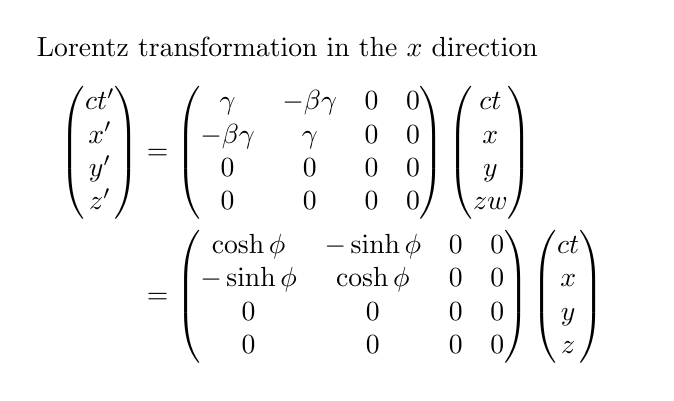
\begin{tikzpicture}[scale=1]
  \node[align=left] at (0,0) {
    \begin{minipage}{7.5cm}
    Lorentz transformation in the $x$ direction
    \begin{align*}
      \begin{pmatrix}
        ct' \\
        x' \\
        y' \\
        z'
      \end{pmatrix}
      &=
      \begin{pmatrix}
        \gamma & -\beta\gamma & 0 & 0 \\
        -\beta\gamma & \gamma & 0 & 0 \\
        0 & 0 & 0 & 0 \\
        0 & 0 & 0 & 0
      \end{pmatrix}
      \begin{pmatrix}
        ct \\
        x \\
        y \\
        zw
      \end{pmatrix}\\
      &=
      \begin{pmatrix}
         \cosh\phi & -\sinh\phi & 0 & 0 \\
        -\sinh\phi &  \cosh\phi & 0 & 0 \\
        0 & 0 & 0 & 0 \\
        0 & 0 & 0 & 0
      \end{pmatrix}
      \begin{pmatrix}
        ct \\
        x \\
        y \\
        z
      \end{pmatrix}
    \end{align*}
    \end{minipage}
  };
\end{tikzpicture}


% SPACETIME DIAGRAM - MULTIPLE INVARIANT HYPERBOLOIDS
% Inspiration: https://commons.wikimedia.org/wiki/File:Spacelike_and_Timelike_Invariant_Hyperbolas.png
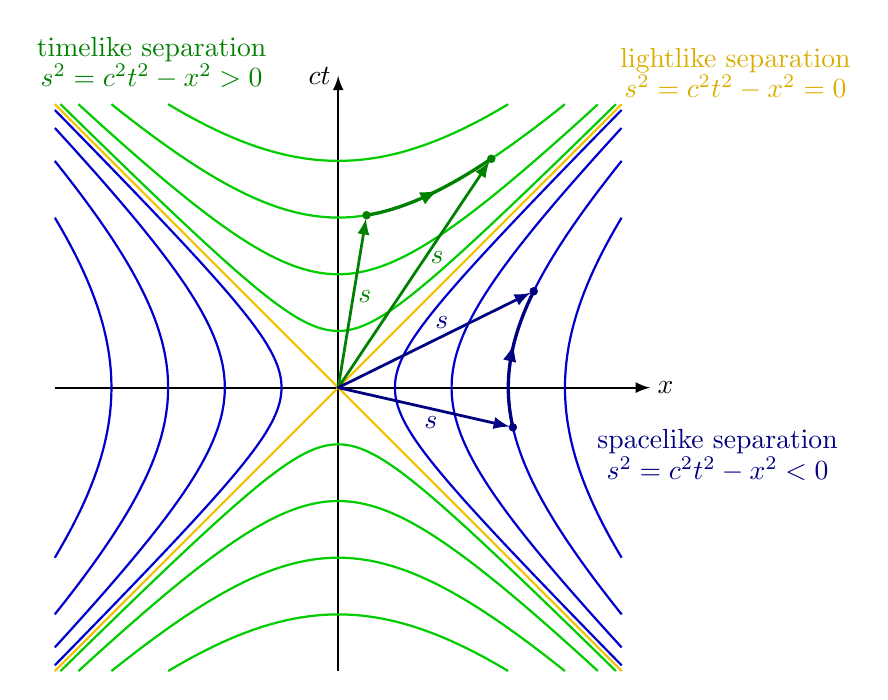
\begin{tikzpicture}[scale=1.8]
  \message{Multiple invariant hyperboloids^^J}
  
  \def\xmax{2}
  \def\Nlines{4} % number of world lines (at constant x/t)
  \pgfmathsetmacro\w{\xmax/(\Nlines+1)}
  
  % AXES
  \draw[->,thick] (0,-\xmax) -- (0,\xmax+0.2) node[left=-1] {$ct$};
  \draw[->,thick] (-\xmax,0) -- (\xmax+0.2,0) node[right=-1] {$x$};
  
  % LIGHTCONE
  \draw[myorange,thick] (-\xmax,-\xmax) -- (\xmax, \xmax);
  \draw[myorange,thick] (-\xmax, \xmax) -- (\xmax,-\xmax);
  
  \foreach \i [evaluate={\s=\xmax*\i/(\Nlines+1); \xm=sqrt(\xmax^2-\s^2);}] in {1,...,\Nlines}{
    
    % SPACELIKE HYPERBOLOIDS
    \draw[mygreen,thick,samples=\Nsamples,smooth,variable=\x,domain=-\xm:\xm]
      plot(\x,-{sqrt(\s^2+(\x)^2)})
      plot(\x,{sqrt(\s^2+(\x)^2)});
    
    % TIMELIKE HYPERBOLOIDS
    \draw[myblue,thick,samples=\Nsamples,smooth,variable=\y,domain=-\xm:\xm]
      plot(-{sqrt(\s^2+(\y)^2)},\y)
      plot({sqrt(\s^2+(\y)^2)},\y);
    
  }
  
  % LABELS
  \node[mydarkgreen,above left=2,align=center] at (-0.2*\xmax,\xmax)
    {timelike separation\\[-1]$s^2 = c^2t^2 - x^2 > 0$};
  \node[mydarkorange,left=2,above right=-2,align=center] at (\xmax,\xmax)
    {lightlike separation\\[-1]$s^2 = c^2t^2 - x^2 = 0$};
  \node[mydarkblue,right=0,align=center] at (0.88*\xmax,-0.24*\xmax)
    {spacelike separation\\[-1]$s^2 = c^2t^2 - x^2 < 0$};
  
  % VECTORS
  \def\xa{0.5}
  \def\xb{2.7}
  \def\ta{-0.7}
  \def\tb{1.7}
  \draw[mydarkgreen,very thick,decoration={markings,mark=at position 0.55 with {\arrow{latex}}},
        postaction={decorate},samples=20,variable=\x,domain=\xa:\xb]
    plot({\w*\x},{\w*sqrt((\x)^2+3^2)});
  \draw[mydarkblue,very thick,decoration={markings,mark=at position 0.6 with {\arrow{latex}}},
        postaction={decorate},samples=20,variable=\x,domain=\ta:\tb]
    plot({\w*sqrt((\x)^2+3^2)},{\w*\x});
  \fill[mydarkgreen] ({\w*\xa},{\w*sqrt(\xa^2+3^2)}) coordinate (A) circle(0.03);
  \fill[mydarkgreen] ({\w*\xb},{\w*sqrt(\xb^2+3^2)}) coordinate (A') circle(0.03);
  \fill[mydarkblue] ({(\w*sqrt((\ta)^2+3^2)},{\w*\ta}) coordinate (B) circle(0.03);
  \fill[mydarkblue] ({(\w*sqrt((\tb)^2+3^2)},{\w*\tb}) coordinate (B') circle(0.03);
  \draw[vector',mydarkgreen] (0,0) -- (A)
    node[pos=0.53,right=-2] {$s$};
  \draw[vector',mydarkgreen] (0,0) -- (A')
    node[pos=0.57,right=-2] {$s$};
  \draw[vector',mydarkblue] (0,0) -- (B)
    node[pos=0.53,below=-1] {$s$};
  \draw[vector',mydarkblue] (0,0) -- (B')
    node[pos=0.53,above=-1] {$s$};
  
\end{tikzpicture}


% ROTATION MATRIX
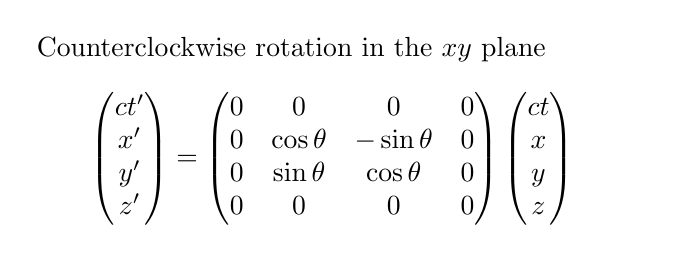
\begin{tikzpicture}[scale=1]
  \node[align=left] at (0,0) {
    \begin{minipage}{7.5cm}
    Counterclockwise rotation in the $xy$ plane
    \begin{align*}
      \begin{pmatrix}
        ct' \\
        x' \\
        y' \\
        z'
      \end{pmatrix}
      &=
      \begin{pmatrix}
        0 & 0 & 0 & 0 \\
        0 & \cos\theta & -\sin\theta & 0 \\
        0 & \sin\theta &  \cos\theta & 0 \\
        0 & 0 & 0 & 0
      \end{pmatrix}
      \begin{pmatrix}
        ct \\
        x \\
        y \\
        z
      \end{pmatrix}
    \end{align*}
    \end{minipage}
  };
\end{tikzpicture}


% SPACE DIAGRAM - MULTIPLE INVARIANT SPHERES (SPACETIME SLICES)
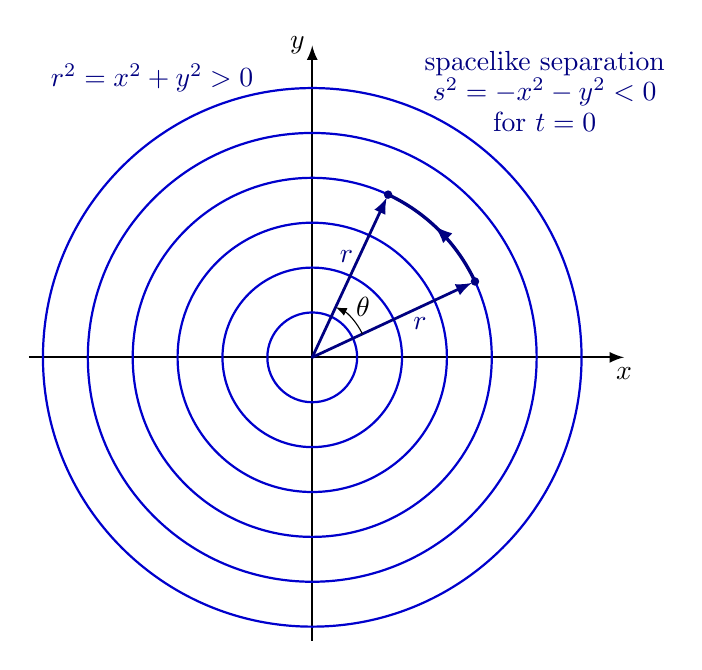
\begin{tikzpicture}[scale=1.8]
  \message{Multiple invariant spheres^^J}
  
  \def\xmax{2}
  \def\Rmax{0.95*\xmax} % outermost radius
  \def\R{\Rmax*4/\Nlines} % radius
  \def\anga{25} % start angle
  \def\angb{65} % end angle
  \def\Nlines{6} % number of world lines (at constant x/t)
  \coordinate (O) at (0,0);
  \coordinate (A) at (\anga:\R);
  \coordinate (B) at (\angb:\R);
  
  % AXES
  \draw[->,thick] (0,-\xmax) -- (0,\xmax+0.2) node[left=-1] {$y$};
  \draw[->,thick] (-\xmax,0) -- (\xmax+0.2,0) node[below=0] {$x$};
  
  % SPACELIKE SPHERES
  \foreach \i [evaluate={\r=\Rmax*\i/\Nlines;}] in {1,...,\Nlines}{
    \draw[myblue,thick] (0,0) circle(\r);
  }
  
  % LABELS
  \fill[mydarkblue] (A) circle(0.03);
  \fill[mydarkblue] (B) circle(0.03);
  \node[mydarkblue,left=0] at (100:\xmax) {$r^2 = x^2 + y^2 > 0$};
  \node[mydarkblue,right=2,align=center] at (70:\xmax)
    {spacelike separation\\[-1]$s^2 = - x^2 - y^2 < 0$\\[-1]for $t=0$};
  \draw[vector',mydarkblue] (0,0) -- (A) node[pos=0.59,below right=-2] {$r$};
  \draw[vector',mydarkblue] (0,0) -- (B) node[pos=0.57,above left=-3] {$r$};
  \draw pic[->,"$\theta$",draw=black,angle radius=20,angle eccentricity=1.3] {angle = A--O--B};
  \draw[mydarkblue,very thick,decoration={markings,mark=at position 0.55 with {\arrow{latex}}},
        postaction={decorate}]
    (A) arc(\anga:\angb:\R);
  
\end{tikzpicture}


% SPACE DIAGRAM - MULTIPLE INVARIANT SPHERES (SPACETIME SLICES)
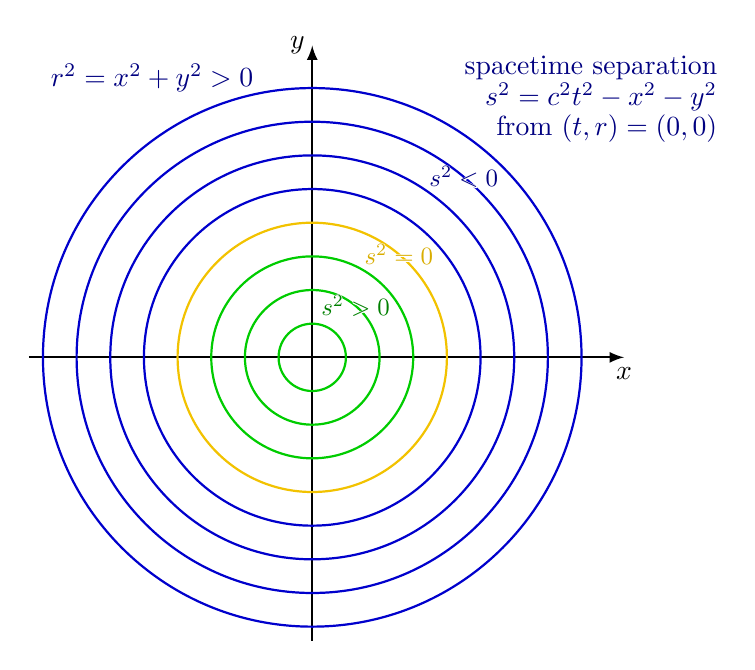
\begin{tikzpicture}[scale=1.8]
  \message{Multiple invariant spheres^^J}
  
  \def\xmax{2}
  \def\Rmax{0.95*\xmax}
  \def\Nlines{8} % number of world lines (at constant x/t)
  
  % AXES
  \draw[->,thick] (0,-\xmax) -- (0,\xmax+0.2) node[left=-1] {$y$};
  \draw[->,thick] (-\xmax,0) -- (\xmax+0.2,0) node[below=0] {$x$};
  
  % SPHERES
  \foreach \i [evaluate={\R=\Rmax*\i/\Nlines;}] in {1,...,3}{
    \draw[mygreen,thick] (0,0) circle(\R); % timelike separation
  }
  \draw[myorange,thick] (0,0) circle(\Rmax*4/\Nlines); % light cone
  \foreach \i [evaluate={\R=\Rmax*\i/\Nlines;}] in {5,...,\Nlines}{
    \draw[myblue,thick] (0,0) circle(\R); % spacelike separation
  }
  
  % LABELS
  \node[mydarkgreen,scale=0.9] at (50:\Rmax*2/\Nlines) {\contour{white}{$s^2>0$}};
  \node[mydarkorange,scale=0.9] at (50:\Rmax*4/\Nlines) {\contour{white}{$s^2=0$}};
  \node[mydarkblue,scale=0.9] at (50:\Rmax*7/\Nlines) {\contour{white}{$s^2<0$}};
  \node[mydarkblue,left=0] at (100:\xmax) {$r^2 = x^2 + y^2 > 0$};
  \node[mydarkblue,right=2,align=right] at (62:1.03*\xmax)
    {spacetime separation\\[-1]$s^2 = c^2t^2 - x^2 - y^2$\\[-1]from $(t,r)=(0,0)$};
  
\end{tikzpicture}


% LORENTZ FACTOR
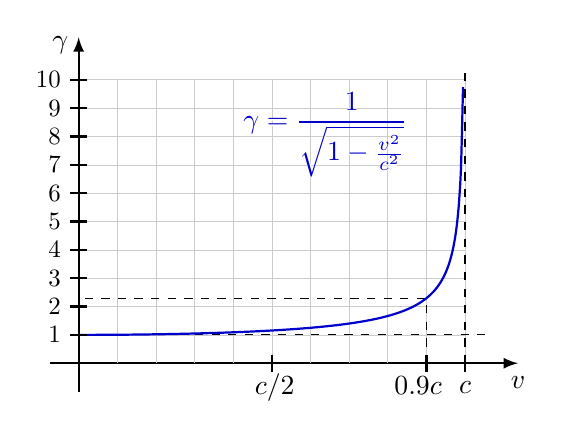
\begin{tikzpicture}[scale=1.8]
  \message{Lorentz factor^^J}
  
  \def\xmax{2.9}
  \def\ymax{2.1}
  \def\A{0.2} % amplitude / y scale
  \pgfmathsetmacro\c{0.94*\xmax} % speed of light
  \coordinate (O) at (0,0);
  
  % AXES
  \draw[->,thick] (-0.2,0) -- (\xmax+0.2,0) node[below=1] {$v$};
  \draw[->,thick] (0,-0.2) -- (0,\ymax+0.2) node[below=3,left=0] {$\gamma$};
  
  % GRID
  \foreach \i in {1,...,10}{
    \draw[black!20,very thin] (0,\i*\A) --++ (\c,0);
    \draw[black!20,very thin] (\i*\c/10,0) --++ (0,10*\A);
  }
  
  % PLOT
  \draw[dashed] (0,\A) --++ (\xmax,0);
  \draw[dashed] (\c,0) --++ (0,\ymax);
  \draw[dashed] (0.9*\c,0) |- (0,{\A/sqrt(1-0.9^2)});
  \draw[myblue,thick,samples=2*\Nsamples,smooth,variable=\v,domain=0:{\c*sqrt(1-(\A/\ymax)^2)}]
    plot(\v,\fpeval{\A/sqrt(1-(\v/\c)^2)});
  \node[myblue,below=1] at (0.6*\xmax,10*\A)
    {\contour{white}{$\gamma=\dfrac{1}{\sqrt{1-\frac{v^2}{c^2}}}$}};
  
  % TICKS
  \tick{\c/2,0}{90} node[right=1,below=-3] {$c/2$};
  \tick{0.9*\c,0}{90} node[left=3,below=-2] {$0.9c$};
  \tick{\c,0}{90} node[below=0] {$c$};
  \foreach \i in {1,...,10}{
    \tick{0,\i*\A}{0} node[left,scale=0.9] {$\i$};
  }
  
\end{tikzpicture}


% LORENTZ FACTOR
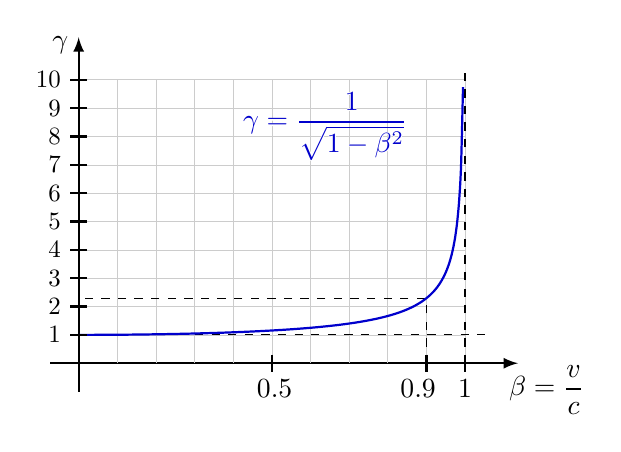
\begin{tikzpicture}[scale=1.8]
  \message{Lorentz factor^^J}
  
  \def\xmax{2.9}
  \def\ymax{2.1}
  \def\A{0.2} % amplitude / y scale
  \pgfmathsetmacro\c{0.94*\xmax} % speed of light
  \coordinate (O) at (0,0);
  
  % AXES
  \draw[->,thick] (-0.2,0) -- (\xmax+0.2,0) node[left=4,below right=-3] {$\beta=\dfrac{v}{c}$};
  \draw[->,thick] (0,-0.2) -- (0,\ymax+0.2) node[below=3,left=0] {$\gamma$};
  
  % GRID
  \foreach \i in {1,...,10}{
    \draw[black!20,very thin] (0,\i*\A) --++ (\c,0);
    \draw[black!20,very thin] (\i*\c/10,0) --++ (0,10*\A);
  }
  
  % PLOT
  \draw[dashed] (0,\A) --++ (\xmax,0);
  \draw[dashed] (\c,0) --++ (0,\ymax);
  \draw[dashed] (0.9*\c,0) |- (0,{\A/sqrt(1-0.9^2)});
  \draw[myblue,thick,samples=2*\Nsamples,smooth,variable=\v,domain=0:{\c*sqrt(1-(\A/\ymax)^2)}]
    plot(\v,\fpeval{\A/sqrt(1-(\v/\c)^2)});
  \node[myblue,below=1] at (0.6*\xmax,10*\A)
    {\contour{white}{$\gamma=\dfrac{1}{\sqrt{1-\beta^2}}$}};
  
  % TICKS
  \tick{\c/2,0}{90} node[right=1,below=-1] {$0.5$};
  \tick{0.9*\c,0}{90} node[left=3,below=-1] {$0.9$};
  \tick{\c,0}{90} node[below=-1] {$1$};
  \foreach \i in {1,...,10}{
    \tick{0,\i*\A}{0} node[left,scale=0.9] {$\i$};
  }
  
\end{tikzpicture}


\end{document}